\chapter{Optimization and Quadratic Forms}

In Chapter~35, we saw electrical networks find currents that minimize dissipated power,
and random walks settle into equilibrium. Both illustrate a universal theme:
many mathematical problems reduce to a search for an optimal configuration.
Examples include finding the best-fit line through a data set, the most efficient
distribution of current through a circuit, the configuration of neural network
weights that minimizes loss, or the shape a soap film adopts to minimize surface area.
In each case, an objective function assigns a real number to every choice -- a cost,
an error, or an energy -- and the goal is to minimize or maximize this value. That is
the core problem of \emph{optimization}.

This chapter rests on one observation. Most of the smooth cost surfaces that actually
matter, at least near their lowest points, look like the same simple shape: a \emph{bowl}.
In Chapter 27 we met the algebraic engine of that bowl: the symmetric matrix $\mat{A}$
acting in the quadratic form $\vec{x}\T\mat{A}\vec{x}$. There we saw that positive
eigenvalues make $\vec{x}\T\mat{A}\vec{x}$ strictly positive. Here we turn that insight
into an algorithm. The geometry of a quadratic form -- bowl, dome, saddle, or trough --
is governed entirely by the eigenvalues and eigenvectors of $\mat{A}$. So the linear
algebra you already know turns out to be the exact language of multivariable curvature,
equilibrium, and constrained optimization.

We will build the picture first, learning to read off from a matrix whether a surface
curves up into a bowl (a minimum), down into a dome (a maximum), or twists into a
saddle (neither). Along the way we will see that ``positive definite'', ``convex'', and
``has a unique global minimum'' are three phrasings of one geometric idea; that least
squares is simply the gradient of an error bowl set to zero; and that constrained
optimization -- whether subject to smooth equality constraints or boundary
inequalities -- connects directly to eigenvalues via Lagrange multipliers and the
Karush--Kuhn--Tucker conditions.

\section{Curved surfaces and their bottoms}
\label{ch36:landscape}

Fix the mental picture once and for all. Imagine a function $f$ that takes a
point $\vec{x}$ in the plane and returns a single height $f(\vec{x})$. Plot that
height as a surface sitting above the plane. Optimization is the question: \emph{over
all points $\vec{x}$, where is the surface lowest?}

\begin{intuitionbox}
Picture a marble rolling on the surface. It rolls downhill and settles at a low
point. The places where it can come to rest are the places where the ground is
\emph{flat} -- no slope in any direction to push the marble along. Those flat spots
are the \emph{critical points}. Most of optimization is two separate questions:
(1) where is the ground flat? and (2) of those flat spots, which are genuine
bottoms (minima), which are tops (maxima), and which are passes that go up one way
and down another (saddles)?
\end{intuitionbox}

The first question is about the \emph{gradient} -- the slope. The second is about
\emph{curvature} -- how the surface bends -- and curvature is where the quadratic
forms live. Here are the three archetypal shapes, because every smooth
surface, zoomed in close enough to a flat spot, looks like one of them.

\begin{figure}[H]
\centering
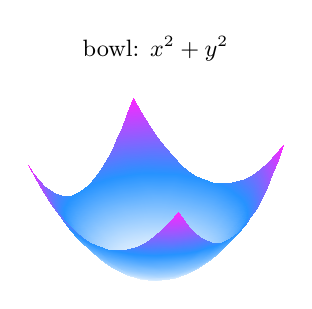
\begin{tikzpicture}[scale=0.95]
\begin{axis}[
  hide axis, width=5.0cm, height=5.0cm, view={35}{30},
  domain=-1.4:1.4, y domain=-1.4:1.4, samples=20,
  title style={font=\small}, title={bowl: $x^2+y^2$}]
  \addplot3[surf,shader=interp,fill opacity=0.85,colormap/cool] {x^2+y^2};
\end{axis}
\end{tikzpicture}
\hspace{0.1cm}
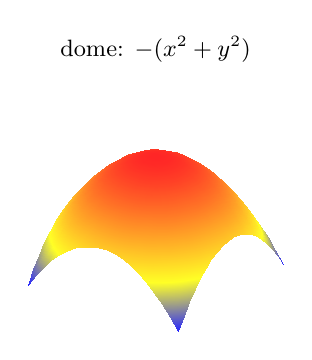
\begin{tikzpicture}[scale=0.95]
\begin{axis}[
  hide axis, width=5.0cm, height=5.0cm, view={35}{30},
  domain=-1.4:1.4, y domain=-1.4:1.4, samples=20,
  title style={font=\small}, title={dome: $-(x^2+y^2)$}]
  \addplot3[surf,shader=interp,fill opacity=0.85,colormap/hot] {-(x^2+y^2)};
\end{axis}
\end{tikzpicture}
\hspace{0.1cm}
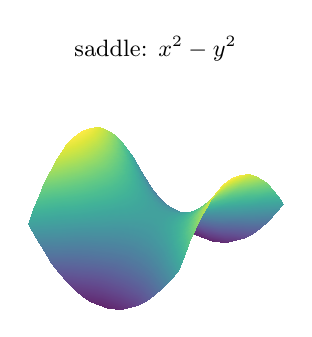
\begin{tikzpicture}[scale=0.95]
\begin{axis}[
  hide axis, width=5.0cm, height=5.0cm, view={35}{30},
  domain=-1.4:1.4, y domain=-1.4:1.4, samples=20,
  title style={font=\small}, title={saddle: $x^2-y^2$}]
  \addplot3[surf,shader=interp,fill opacity=0.85,colormap/viridis] {x^2-y^2};
\end{axis}
\end{tikzpicture}
\caption{The three basic shapes of a quadratic surface. The \emph{bowl} curves up
in every direction (a minimum at the center). The \emph{dome} curves down in every
direction (a maximum). The \emph{saddle} curves up along one axis and down along
another (neither). Reading which one you have from the eigenvalues of its matrix is the
first key step in multivariable optimization.}
\label{ch36:fig-three-shapes}
\end{figure}

The three formulas under those pictures -- $x^2+y^2$, $-(x^2+y^2)$, $x^2-y^2$ -- are
our first quadratic forms. Notice they are built only from \emph{squares and
products} of the coordinates: $x^2$, $y^2$, $xy$. No lonely $x$ or $y$ term, no
constant. That is the defining feature, and it is exactly the kind of expression a
symmetric matrix produces.

\section{Quadratic forms: \texorpdfstring{$\vec{x}\T\mat{A}\vec{x}$}{x'Ax}}
\label{ch36:quadforms}

In Chapter 27, we introduced the quadratic form as an energy test for positive
definite matrices. Let us briefly revisit how the matrix builds the polynomial,
keeping our eyes focused now on the geometry of slopes, level curves, and algorithms.
Take a symmetric $2\times 2$ matrix and sandwich it between a column vector on the
right and its transpose (a row vector) on the left:
\[
  \vec{x}\T\mat{A}\vec{x}
  = \begin{bmatrix} x & y \end{bmatrix}
    \begin{bmatrix} a & b \\ b & c \end{bmatrix}
    \colvec{x \\ y}.
\]
Multiply it out carefully. First the matrix times the vector:
\[
  \begin{bmatrix} a & b \\ b & c \end{bmatrix}\colvec{x\\y}
  = \colvec{ax+by \\ bx+cy}.
\]
Then the row vector times that:
\[
  \begin{bmatrix} x & y \end{bmatrix}\colvec{ax+by\\bx+cy}
  = x(ax+by) + y(bx+cy)
  = a x^2 + 2b\,xy + c y^2.
\]
There it is. The sandwich $\vec{x}\T\mat{A}\vec{x}$ collapses to a tidy polynomial in
which every term has total degree exactly two. The diagonal entries $a,c$ become the
pure-square coefficients; the off-diagonal entry $b$ becomes the coefficient of the
cross term $xy$, doubled because it appears in both off-diagonal slots.

\begin{definition}[Quadratic form]
\label{ch36:def-qform}
Let $\mat{A}$ be an $n\times n$ symmetric matrix. The function
\[
  Q(\vec{x}) \;=\; \vec{x}\T\mat{A}\vec{x} \;=\; \sum_{i=1}^{n}\sum_{j=1}^{n} A_{ij}\,x_i x_j
\]
is the \emph{quadratic form} associated with $\mat{A}$. It maps a vector $\vec{x}\in
\R^n$ to a single real number, and every term is degree two in the coordinates.
\end{definition}

\begin{focusbox}
A quadratic form is the matrix world's version of ``$y = a x^2$.'' One number $a$
tells you whether the parabola opens up or down and how sharply. A whole symmetric
matrix $\mat{A}$ tells you the same thing in many dimensions at once: which
directions open up, which open down, and how sharply in each.
\end{focusbox}

\subsection{Why symmetric, and why the factor of two}

You might worry: what if the matrix is not symmetric? Suppose $\mat{M}$ has
off-diagonal entries $p$ (top right) and $q$ (bottom left) that differ. Working out
$\vec{x}\T\mat{M}\vec{x}$ gives $a x^2 + (p+q)xy + c y^2$. Only the \emph{sum} $p+q$
survives -- the form cannot tell $p=1,q=3$ from $p=q=2$. So for any matrix we could
replace it by its ``symmetric part'' $\tfrac12(\mat{M}+\mat{M}\T)$ without changing
the form at all. Since the quadratic form only ever sees the symmetric part, we lose
nothing by \emph{always} taking $\mat{A}$ symmetric, and we gain a great deal: the
spectral theory of symmetric matrices (real eigenvalues, orthogonal
eigenvectors) becomes available to read the geometry.

\begin{trapbox}
The factor of $2$ trips everyone up once. If you want the cross-term $6xy$ in your
form, the matrix entry $b$ is \emph{half} of that, $b=3$, because $b$ appears twice
(top-right and bottom-left) and the two copies add. So
\[
  3x^2 + 6xy + 5y^2 \;\longleftrightarrow\; \mat{A}=\begin{bmatrix}3 & 3\\ 3 & 5\end{bmatrix},
  \quad\text{not } \begin{bmatrix}3&6\\6&5\end{bmatrix}.
\]
Always halve the cross-term coefficient when you build the matrix; always double the
off-diagonal when you read the form back out.
\end{trapbox}

\begin{labbox}
Build the symmetric matrix for each form, then read it back to check.
(a) $2x^2 + 4xy + 7y^2$. (b) $x^2 - 6xy + y^2$. (c) $5x^2 + 5y^2$ (no cross term).
(d) In three variables, $x^2 + y^2 + z^2 + 2xy + 2yz$ -- careful, there is no $xz$
term, so the $(1,3)$ entry is $0$. Answers:
(a) $\begin{bmatrix}2&2\\2&7\end{bmatrix}$;
(b) $\begin{bmatrix}1&-3\\-3&1\end{bmatrix}$;
(c) $\begin{bmatrix}5&0\\0&5\end{bmatrix}$;
(d) $\begin{bmatrix}1&1&0\\1&1&1\\0&1&1\end{bmatrix}$.
\end{labbox}

\subsection{A first worked form and its level curves}

Take $\mat{A}=\begin{bmatrix}3&0\\0&1\end{bmatrix}$, a diagonal matrix, so its form
is $Q(x,y)=3x^2+y^2$ with no cross term. Where is $Q$ equal to a constant, say
$Q=3$? That is the equation $3x^2+y^2=3$, i.e. $x^2 + y^2/3 = 1$ -- an ellipse,
short in the $x$-direction (radius $1$) and tall in the $y$-direction (radius
$\sqrt 3$). Set $Q=12$ and you get a bigger ellipse of the same shape. The level
curves are a nested family of ellipses, all centered at the origin, and the surface
$z=Q(x,y)$ is a bowl whose cross-sections are exactly these ellipses.

\begin{figure}[H]
\centering
\begin{tikzpicture}[scale=1.0,>=Latex]
  \draw[help lines,gray!25] (-2.6,-2.6) grid (2.6,2.6);
  \draw[->] (-2.7,0)--(2.7,0) node[right]{$x$};
  \draw[->] (0,-2.7)--(0,2.7) node[above]{$y$};
  % ellipses 3x^2 + y^2 = k : semi-axes sqrt(k/3) in x, sqrt(k) in y
  \draw[vecblue,thick]  (0,0) ellipse ({sqrt(1)} and {sqrt(3)});   % k=3
  \draw[vecblue,thick]  (0,0) ellipse ({sqrt(2)} and {sqrt(6)});   % k=6
  \node[vecblue,font=\small] at (2.1,1.35) {$Q{=}3$};
  \draw[->,vecblue,thin] (1.6,1.15) -- (0.95,0.8);
  % principal axes
  \draw[->,vecred,very thick] (0,0)--(1,0);
  \node[vecred, font=\scriptsize, align=center] at (0.45,-0.38) {steep\\axis};
  \draw[->,targetgreen,very thick] (0,0)--(0,1.732);
  \node[targetgreen, left=2pt, font=\small] at (0,0.9) {gentle axis};
\end{tikzpicture}
\caption{Level curves of $Q(x,y)=3x^2+y^2$. Each blue curve is a set $Q=\text{const}$,
an ellipse. The form grows \emph{fastest} along the short $x$-axis (eigenvalue $3$)
and \emph{slowest} along the long $y$-axis (eigenvalue $1$): big eigenvalue means
steep wall, so the ellipse is squeezed in that direction.}
\label{ch36:fig-levelcurves}
\end{figure}

Notice the eigenvalues of this diagonal matrix are $3$ and $1$, sitting right on the
diagonal, with eigenvectors along the axes. The big eigenvalue $3$ goes with the
\emph{steep} direction (the wall of the bowl rises fast, so the ellipse is short
there); the small eigenvalue $1$ goes with the \emph{gentle} direction. This is the
whole secret of quadratic-form geometry, and it survives even when the matrix is not
diagonal -- we just have to rotate to the eigenvector axes first.

\begin{recoverybox}
\textbf{Mental check: reading the shape.} If $Q(x,y) = 5x^2 + 2y^2$, what are the
semi-axes of the ellipse $Q(x,y) = 10$? In the $x$-direction, $5x^2 = 10 \Rightarrow
x = \pm\sqrt{2}$. In the $y$-direction, $2y^2 = 10 \Rightarrow y = \pm\sqrt{5}$. The
ellipse is wider in $y$ ($\sqrt{5} \approx 2.24$) and narrower in $x$ ($\sqrt{2}
\approx 1.41$). Why is it narrower along $x$? Because the coefficient $5$ is larger:
the bowl rises more steeply in $x$, so the contour height $10$ is reached much closer
to the origin.
\end{recoverybox}

\section{Diagonalizing the form: the principal axes}
\label{ch36:principal-axes}

What if there is a cross term? Take
\[
  \mat{A}=\begin{bmatrix} 2 & 1 \\ 1 & 2 \end{bmatrix},
  \qquad Q(x,y) = 2x^2 + 2xy + 2y^2.
\]
The level curves $Q=\text{const}$ are still ellipses, but now they are \emph{tilted}
-- their axes do not line up with the coordinate axes, precisely because of the $xy$
term. The cross term is the algebraic fingerprint of a tilt. To visualize the bowl's principal geometry
we want to rotate our coordinates until the tilt vanishes. And we already know how:
diagonalize the symmetric matrix.

Recall from the spectral theorem that a symmetric matrix factors as
$\mat{A}=\mat{Q}\mat{\Lambda}\mat{Q}\T$, where $\mat{Q}$ is orthogonal (its columns
are orthonormal eigenvectors) and $\mat{\Lambda}=\diag(\lambda_1,\dots,\lambda_n)$
holds the eigenvalues. For our $\mat{A}$ the eigenvalues are $3$ and $1$ with
eigenvectors $\tfrac{1}{\sqrt2}\colvec{1\\1}$ and $\tfrac{1}{\sqrt2}\colvec{1\\-1}$
(you verified these back in the eigenvalue chapter). Now substitute the factorization
into the form and introduce \emph{new coordinates} $\vec{y}=\mat{Q}\T\vec{x}$ -- the
coordinates of $\vec{x}$ in the eigenvector frame:
\[
  Q(\vec{x}) = \vec{x}\T\mat{A}\vec{x}
  = \vec{x}\T \mat{Q}\mat{\Lambda}\mat{Q}\T \vec{x}
  = (\mat{Q}\T\vec{x})\T \mat{\Lambda} (\mat{Q}\T\vec{x})
  = \vec{y}\T \mat{\Lambda}\vec{y}
  = \lambda_1 y_1^2 + \lambda_2 y_2^2.
\]
The cross term is gone. In the rotated coordinates the form is purely a sum of
weighted squares, and the weights are the eigenvalues. This is the \emph{principal
axes theorem}, and most of the rest of the chapter leans on it.

\begin{formalbox}
\label{ch36:thm-principal-axes}
\textbf{Principal axes theorem.} Let $\mat{A}$ be symmetric with eigenvalues $\lambda_1,\dots,\lambda_n$ and an
orthonormal eigenbasis forming the columns of an orthogonal matrix $\mat{Q}$. In the
rotated coordinates $\vec{y}=\mat{Q}\T\vec{x}$,
\[
  \vec{x}\T\mat{A}\vec{x} \;=\; \lambda_1 y_1^2 + \lambda_2 y_2^2 + \cdots + \lambda_n y_n^2.
\]
Every quadratic form is, in the right rotated frame, a weighted sum of pure squares.
The eigenvectors point along the principal axes of the level-set ellipsoids; the
eigenvalues control how far those axes stretch.
\end{formalbox}

\begin{figure}[H]
\centering
\begin{tikzpicture}[scale=1.05,>=Latex]
  \draw[help lines,gray!25] (-2.4,-2.4) grid (2.4,2.4);
  \draw[->] (-2.5,0)--(2.5,0) node[right]{$x$};
  \draw[->] (0,-2.5)--(0,2.5) node[above]{$y$};
  % Tilted ellipse: Q = 2x^2+2xy+2y^2 = k, principal axes at 45 deg.
  % In eigen-coords: 3 u^2 + 1 v^2 = k. For k=3: u-axis radius 1, v-axis radius sqrt3.
  \begin{scope}[rotate=45]
    \draw[vecblue,thick] (0,0) ellipse ({1} and {1.732});
    \draw[vecblue,thick] (0,0) ellipse ({1.414} and {2.449});
  \end{scope}
  % eigen-axes
  \draw[->,vecred,very thick] (0,0)--(0.707,0.707) node[above right]{\small $\lambda{=}3$ (steep)};
  \draw[->,targetgreen,very thick] (0,0)--(0.707,-0.707) node[below right]{\small $\lambda{=}1$ (gentle)};
\end{tikzpicture}
\caption{The form $2x^2+2xy+2y^2$ has \emph{tilted} elliptical level curves. The
cross term rotated the picture by $45^\circ$. The eigenvectors $\colvec{1\\1}$ and
$\colvec{1\\-1}$ are the principal axes; the bowl is steepest along the eigenvalue-$3$
direction and gentlest along the eigenvalue-$1$ direction.}
\label{ch36:fig-tilted}
\end{figure}

\begin{aestheticbox}
Pause on how much this collapses. A general symmetric $n\times n$ form has up to
$n(n+1)/2$ independent coefficients -- a messy soup of squares and cross terms. The
principal axes theorem says: \emph{in the right orthonormal frame, all of that is
just $n$ numbers, the eigenvalues, stretching $n$ perpendicular axes.} Curvature in
many dimensions, which sounds impossibly complicated, is simply a handful of
independent one-dimensional parabolas glued together at right angles. This expresses
the core message of diagonalization in geometric terms: rotating to the eigenbasis
decouples the coordinate directions.
\end{aestheticbox}

\section{Reading the shape: definiteness}
\label{ch36:definiteness}

Now we can answer the question the whole chapter is built around. Look at the
diagonal form $\lambda_1 y_1^2 + \cdots + \lambda_n y_n^2$. Its sign at any nonzero
$\vec{y}$ is controlled entirely by the signs of the eigenvalues.

\begin{itemize}
\item If \emph{every} $\lambda_i>0$, then every term is positive (for $\vec{y}\ne
\vec{0}$), so $Q>0$ always. The surface is a genuine \textbf{bowl}: a minimum at the
origin. We call $\mat{A}$ \emph{positive definite}.
\item If every $\lambda_i<0$, then $Q<0$ always: a \textbf{dome}, a maximum.
\emph{Negative definite}.
\item If the eigenvalues have \emph{mixed} signs -- some positive, some negative --
then $Q$ goes up along some axes and down along others: a \textbf{saddle}.
\emph{Indefinite}.
\item If some eigenvalue is $0$ (and the rest share a sign), the form flattens out
along that axis -- a trough or ridge rather than a strict bowl. \emph{Positive (or
negative) semidefinite}.
\end{itemize}

\begin{formalbox}
\label{ch36:thm-definiteness}
\textbf{Definiteness via eigenvalues.} For a symmetric matrix $\mat{A}$ with eigenvalues $\lambda_1,\dots,\lambda_n$:
\[
\begin{array}{ll}
\text{positive definite} & \iff \text{all } \lambda_i > 0 \iff \vec{x}\T\mat{A}\vec{x} > 0 \text{ for all } \vec{x}\ne\vec{0},\\[2pt]
\text{positive semidefinite} & \iff \text{all } \lambda_i \ge 0,\\[2pt]
\text{negative definite} & \iff \text{all } \lambda_i < 0,\\[2pt]
\text{indefinite} & \iff \text{some } \lambda_i>0 \text{ and some } \lambda_j<0.
\end{array}
\]
\end{formalbox}

\begin{strangbox}
Strang devotes a whole chapter to positive definite matrices, and he loves to give
the energy test $\vec{x}\T\mat{A}\vec{x}>0$ as the \emph{definition}, with the
eigenvalue test and the pivot test as equivalent ``tests.'' Reading this chapter
before Strang, hold onto the geometry: positive definite \emph{means} the surface is
a bowl, so optimization works. Reading it after Strang, you now see why he cared so
much -- the bowl is exactly the surface on which Newton's method, conjugate
gradients, and every clean convex algorithm converge.
\end{strangbox}

\subsection{Checking definiteness without computing eigenvalues}

Computing eigenvalues is work. For $2\times 2$ matrices there is a lightning-fast
test using the trace and determinant. The eigenvalues satisfy $\lambda_1\lambda_2=
\det\mat{A}$ and $\lambda_1+\lambda_2=\tr\mat{A}$. So:

\begin{itemize}
\item $\det\mat{A}>0$ means the eigenvalues share a sign (their product is
positive). Then the trace tells you which: $\tr\mat{A}>0 \Rightarrow$ both positive
$\Rightarrow$ \emph{positive definite}; $\tr\mat{A}<0 \Rightarrow$ both negative
$\Rightarrow$ negative definite.
\item $\det\mat{A}<0$ means the eigenvalues have opposite signs $\Rightarrow$
\emph{indefinite}, a saddle.
\end{itemize}

\begin{example}[The trace--determinant test in action]
\label{ch36:ex-tracedet}
For $\mat{A}=\begin{bmatrix}2&1\\1&2\end{bmatrix}$: $\det=4-1=3>0$ and $\tr=4>0$, so
positive definite -- a bowl. Indeed its eigenvalues were $3,1$. For
$\mat{B}=\begin{bmatrix}1&2\\2&1\end{bmatrix}$: $\det=1-4=-3<0$, so indefinite -- a
saddle (eigenvalues $3$ and $-1$). Two innocent-looking matrices, just an entry
swapped, with completely different geometry: one a bowl, the other a saddle.
\end{example}

For larger matrices the clean generalization is \emph{Sylvester's criterion}: a
symmetric matrix is positive definite exactly when all its \emph{leading principal
minors} -- the determinants of the top-left $1\times1$, $2\times2$, \dots, $n\times
n$ blocks -- are positive. This criterion directly reflects the pivot test: each positive
minor guarantees one positive pivot in elimination, and positive pivots correspond to
positive eigenvalues.

\begin{example}[A $3\times 3$ check by minors]
\label{ch36:ex-minors}
Test $\mat{A}=\begin{bmatrix} 2&-1&0\\ -1&2&-1\\ 0&-1&2\end{bmatrix}$ (it will reappear
as a famous matrix below). Leading minors: $|2|=2>0$;
$\det\begin{bmatrix}2&-1\\-1&2\end{bmatrix}=3>0$; and the full determinant is
$2(4-1)-(-1)(-2-0)=6-2=4>0$. All positive, so $\mat{A}$ is positive definite. Its
form $2x^2+2y^2+2z^2-2xy-2yz$ is a $3$-D bowl.
\end{example}

\begin{trapbox}
Positive \emph{diagonal entries do not} make a matrix positive definite. The diagonal
entries are just $\vec{e}_i\T\mat{A}\vec{e}_i$, the values of the form along the
coordinate axes -- they say nothing about diagonal directions. The matrix
$\begin{bmatrix}1&2\\2&1\end{bmatrix}$ has positive diagonal yet is indefinite. You
must check the off-diagonal pull, which is what the determinant minors do.
\end{trapbox}

\section{Gradients, Hessians, and where the marble stops}
\label{ch36:gradient-hessian}

Time to connect the static picture of forms to the dynamic act of \emph{finding} a
minimum of a general (not necessarily quadratic) function $f(\vec{x})$. Two objects
do all the work.

The \textbf{gradient} $\nabla f$ collects the partial derivatives into a vector:
\[
  \nabla f(\vec{x}) = \colvec{\partial f/\partial x_1 \\ \vdots \\ \partial f/\partial x_n}.
\]
Geometrically it points in the direction of \emph{steepest ascent}, and its length is
the steepness. At a flat spot -- a candidate minimum or maximum -- the ground has no
slope, so $\nabla f=\vec{0}$. That is the first-order condition.

\begin{focusbox}
\emph{First-order condition (stationarity).} At any minimum or maximum in the
interior, $\nabla f(\vec{x}^\star)=\vec{0}$. Setting the gradient to zero is how we
\emph{find} candidate optima. But a zero gradient alone cannot tell bowl from dome
from saddle -- for that we need curvature.
\end{focusbox}

The \textbf{Hessian} $\mat{H}$ is the matrix of second partial derivatives:
\[
  \mat{H}(\vec{x}) = \begin{bmatrix}
   \dfrac{\partial^2 f}{\partial x_1^2} & \cdots & \dfrac{\partial^2 f}{\partial x_1\partial x_n}\\[8pt]
   \vdots & \ddots & \vdots\\[4pt]
   \dfrac{\partial^2 f}{\partial x_n\partial x_1} & \cdots & \dfrac{\partial^2 f}{\partial x_n^2}
  \end{bmatrix}.
\]
Because mixed partials are equal (for nice functions), $\mat{H}$ is automatically \emph{symmetric}.
The Hessian is the symmetric matrix whose quadratic form
\emph{is} the local curvature of $f$. Here is the bridge, written precisely.

\begin{formalbox}
\label{ch36:thm-taylor}
\textbf{Second-order Taylor expansion.} Near a stationary point $\vec{x}^\star$ (where $\nabla f=\vec{0}$), with
$\vec{h}=\vec{x}-\vec{x}^\star$,
\[
  f(\vec{x}^\star+\vec{h}) \;\approx\; f(\vec{x}^\star) \;+\; \underbrace{\nabla f(\vec{x}^\star)\T\vec{h}}_{=\,0}
  \;+\; \tfrac12\,\vec{h}\T\mat{H}(\vec{x}^\star)\,\vec{h}.
\]
So up to a constant, the surface near a flat spot \emph{is} the quadratic form of its
Hessian. The bowl/dome/saddle classification of the form transfers directly to the
function.
\end{formalbox}

\begin{intuitionbox}
The gradient finds the flat spots; the Hessian reads the local shape there. This is
exactly the single-variable second-derivative test you already know -- ``$f'=0$ and
$f''>0$ means a minimum'' -- promoted to many dimensions, with the scalar $f''>0$
replaced by the matrix statement ``$\mat{H}$ is positive definite.''
\end{intuitionbox}

\begin{historybox}
In 1847, Augustin-Louis Cauchy introduced gradient descent while calculating the astronomical orbits of celestial bodies and comets. Cauchy realized that stepping in the direction of the negative gradient $-\nabla f$ guarantees an immediate decrease in function height. But he was quickly halted by a severe geometric trap: in long, narrow ravines where one direction is steep and the perpendicular direction is shallow, steepest descent bounces back and forth between the ravine walls instead of marching down the valley floor.

For a century, Newton's method offered the textbook fix by using the second-derivative Hessian matrix $\mat{H}$ to divide out curvature and leap straight to the bottom: $\Delta\vec{x} = -\mat{H}\inv \nabla f$. But storing and inverting an $n \times n$ Hessian costs $\mathcal{O}(n^3)$ operations and consumes $n^2$ memory words, an impossible barrier for early computers when $n$ reached thousands of variables. Worse, near a saddle point where the Hessian has negative eigenvalues, Newton's step can launch the search uphill toward a maximum.

In 1952, Magnus Hestenes and Eduard Stiefel resolved this computational bottleneck by inventing the \textbf{Conjugate Gradient (CG)} method for symmetric positive-definite systems. Armed with the spectral geometry of quadratic forms, they constructed search directions that are mutually orthogonal with respect to the energy matrix: $\vec{d}_i\T\mat{A}\vec{d}_j = 0$. Each step completely eliminates error along an entire principal axis of the elliptical bowl without disturbing progress made in earlier steps. CG reaches high precision in only $\mathcal{O}(\sqrt{\kappa} \log(1/\epsilon))$ matrix-vector multiplications without ever storing an inverse matrix, enabling the simulation of large-scale physical structures and fluid flows.

Meanwhile, a second optimization revolution was unfolding around inequality constraints. In 1939, a young graduate student at the University of Chicago named William Karush derived the foundational conditions for inequality-constrained optimization in his master's thesis. But World War II dispersed mathematicians into war research, and Karush's thesis sat unpublished and forgotten in the university library. Twelve years later, in 1951, Harold Kuhn and Albert W. Tucker independently rediscovered and published the identical conditions at Princeton, showing how Lagrange multipliers apply to solid boundary walls. When Kuhn later discovered Karush's 1939 thesis, he and Tucker ensured historical justice by championing Karush's priority, permanently renaming the result the \textbf{Karush--Kuhn--Tucker (KKT)} conditions. The KKT conditions provided the foundation for modern mathematical programming, economic game theory, and machine learning algorithms such as support vector machines.

Today, an active frontier is high-dimensional non-convex optimization. In machine
learning models with billions of parameters, cost surfaces contain saddle points where
gradients vanish but Hessians have mixed eigenvalues. Explaining when gradient methods
avoid saddles, and finding efficient algorithms for non-convex quadratic programming
(which is NP-hard), remain open questions.
\end{historybox}

\begin{formalbox}
\label{ch36:thm-second-order}
\textbf{Second-order conditions.} Suppose $\nabla f(\vec{x}^\star)=\vec{0}$ and let $\mat{H}=\mat{H}(\vec{x}^\star)$.
\[
\begin{array}{ll}
\mat{H} \text{ positive definite} & \Rightarrow\ \text{strict local minimum (bowl),}\\
\mat{H} \text{ negative definite} & \Rightarrow\ \text{strict local maximum (dome),}\\
\mat{H} \text{ indefinite} & \Rightarrow\ \text{saddle point (no extremum),}\\
\mat{H} \text{ semidefinite (a zero eigenvalue)} & \Rightarrow\ \text{inconclusive; look higher.}
\end{array}
\]
\end{formalbox}

\begin{example}[Finding and classifying critical points]
\label{ch36:ex-critical}
Let $f(x,y) = x^2 + xy + y^2 - 3y$. The gradient is
\[
  \nabla f = \colvec{2x + y \\ x + 2y - 3}.
\]
Set it to zero: $2x+y=0$ gives $y=-2x$; substitute into $x+2y-3=0$ to get
$x-4x-3=0$, so $x=-1$, $y=2$. The lone critical point is $(-1,2)$. The Hessian is the
constant matrix
\[
  \mat{H} = \begin{bmatrix} 2 & 1 \\ 1 & 2 \end{bmatrix},
\]
whose $\det=3>0$ and $\tr=4>0$: positive definite. So $(-1,2)$ is a strict minimum.
We did not even need the eigenvalues -- the trace--determinant test settled it. (And
because $\mat{H}$ is constant, this minimum is the \emph{global} one, as the next
section explains.)
\end{example}

\begin{example}[A saddle]
\label{ch36:ex-saddle}
Let $g(x,y)=x^2 - y^2 + 2x$. Then $\nabla g=\colvec{2x+2\\-2y}=\vec0$ at $(-1,0)$,
and $\mat{H}=\begin{bmatrix}2&0\\0&-2\end{bmatrix}$, indefinite ($\det=-4<0$). The
point $(-1,0)$ is a saddle: walk along $x$ and you climb, walk along $y$ and you
descend. A marble placed exactly there is balanced but unstable.
\end{example}

\begin{walkbox}
Take a function you can picture, like the height of a mountain pass. Stand at the
saddle of the pass. In your mind, walk a tiny step in four directions: toward each
peak (uphill) and down each valley (downhill). That up-one-way, down-the-other
feeling \emph{is} indefiniteness -- the Hessian has one positive and one negative
eigenvalue, pointing along the ridge and along the trail. Where exactly do the
positive and negative eigenvector directions point on a real mountain pass?
\end{walkbox}

\section{Positive definite means convex means one bottom}
\label{ch36:convexity}

For a \emph{quadratic} function the Hessian is the same matrix everywhere -- the
curvature never changes. That is what makes quadratic bowls so well behaved: if the
Hessian is positive definite, the function is a single perfect bowl with exactly one
minimum, no other critical points, no surprises. Let us make ``single perfect bowl''
precise with the word \emph{convex}.

\begin{definition}[Convex function]
\label{ch36:def-convex}
A function $f$ is \emph{convex} if for any two points $\vec{x},\vec{z}$ and any
$t\in[0,1]$,
\[
  f\big(t\vec{x} + (1-t)\vec{z}\big) \;\le\; t f(\vec{x}) + (1-t) f(\vec{z}).
\]
Geometrically: the chord joining any two points on the graph lies \emph{on or above}
the graph. The surface never bulges above its own secant lines -- it always cups
upward.
\end{definition}

\begin{figure}[H]
\centering
\begin{tikzpicture}[scale=1.0,>=Latex]
  % convex curve y = 0.6 x^2
  \draw[->] (-2.3,0)--(2.6,0) node[right]{$x$};
  \draw[->] (0,-0.3)--(0,3.0) node[above]{$f$};
  \draw[vecblue,very thick,domain=-2.1:2.1,smooth,samples=60] plot (\x,{0.6*\x*\x});
  % a chord
  \coordinate (P) at (-1.6,{0.6*1.6*1.6});
  \coordinate (Pz) at (1.9,{0.6*1.9*1.9});
  \draw[trapred,thick] (P)--(Pz);
  \fill[trapred] (P) circle (1.6pt) (Pz) circle (1.6pt);
  \node[trapred] at (1.1,2.55) {\small chord above graph};
  \node[vecblue] at (-1.95,2.3) {\small convex $f$};
\end{tikzpicture}
\caption{Convexity: every chord (red) lies on or above the graph (blue). A
positive-definite quadratic is convex in every direction at once, which is why it has
exactly one lowest point and downhill always leads there.}
\label{ch36:fig-convex}
\end{figure}

The connection back to our matrices is exact.

\begin{theorem}[PD Hessian $\Leftrightarrow$ convex quadratic]
\label{ch36:thm-convex}
A quadratic function $f(\vec{x})=\tfrac12\vec{x}\T\mat{A}\vec{x} - \vec{b}\T\vec{x}+c$
with symmetric $\mat{A}$ is convex if and only if $\mat{A}$ is positive
semidefinite, and \emph{strictly} convex (a unique global minimum) if and only if
$\mat{A}$ is positive definite. More generally, a twice-differentiable function is
convex if and only if its Hessian is positive semidefinite \emph{everywhere}.
\end{theorem}

\begin{proof}[Why, in one line of algebra]
Convexity of a twice-differentiable function is equivalent to its second derivative
being nonnegative along every line. Along the line $\vec{x}(t)=\vec{p}+t\vec{d}$, the
second derivative of $f$ is $\frac{d^2}{dt^2}f = \vec{d}\T\mat{H}\vec{d}$. Demanding
this be $\ge 0$ for every direction $\vec{d}$ is \emph{exactly} the definition of
$\mat{H}$ positive semidefinite. For the quadratic, $\mat{H}=\mat{A}$ is constant, so
one check settles convexity globally; positive definiteness ($>0$ strictly) forces a
single bottom.
\end{proof}

\begin{aestheticbox}
This is why linear algebra sits at the center of optimization. ``Convex'' is the
dividing line between problems we can solve reliably and problems that hide local
traps. And convex, for the smooth quadratic-like surfaces that dominate science and
machine learning, \emph{means positive definite Hessian} -- an eigenvalue condition.
Three vocabularies -- the analyst's ``convex,'' the optimizer's ``unique global
minimum,'' the algebraist's ``positive definite'' -- name a single geometric fact:
the surface is a bowl.
\end{aestheticbox}

\subsection{Solving the bowl directly}

For a convex quadratic $f(\vec{x})=\tfrac12\vec{x}\T\mat{A}\vec{x}-\vec{b}\T\vec{x}$
with $\mat{A}$ positive definite, we do not need to roll downhill at all -- we can
jump straight to the bottom. Set the gradient to zero. Differentiating,
\[
  \nabla f(\vec{x}) = \mat{A}\vec{x} - \vec{b} \;=\; \vec{0}
  \quad\Longrightarrow\quad \boxed{\;\mat{A}\vec{x} = \vec{b}.\;}
\]
The minimizer of the bowl is the solution of a linear system. Read that backwards and
it is startling: \emph{solving $\mat{A}\vec{x}=\vec{b}$ is the same as finding the
bottom of an energy bowl.} This is the variational view of linear systems -- the one
that underlies the finite-element method, where physical equilibria are computed by
minimizing energy, and the conjugate-gradient algorithm, which solves $\mat{A}\vec{x}
=\vec{b}$ by literally rolling toward the bottom of this bowl.

\begin{connectionbox}
The bridge to calculus and physics goes further than it first appears. In mechanics, a system at rest sits at
a minimum of potential energy; the condition ``$\nabla(\text{energy})=0$'' is the
equilibrium equation, and stability is the Hessian being positive definite. In
differential equations, the matrix $\mat{A}=\begin{bmatrix}2&-1&0\\-1&2&-1\\0&-1&2\end{bmatrix}$
from Example~\ref{ch36:ex-minors} is the discrete second-derivative operator; its
positive definiteness is the discrete statement that $-\,u''$ stores energy. The
quadratic form $\tfrac12\vec{x}\T\mat{A}\vec{x}$ is a discretized
$\int \tfrac12 (u')^2$. Optimization, linear systems, and the calculus of variations
are one subject seen from three sides.
\end{connectionbox}

\section{Least squares is the gradient of a bowl}
\label{ch36:least-squares}

You met least squares as projection: to ``solve'' an overdetermined system
$\mat{A}\vec{x}=\vec{b}$ with no exact solution, find the $\vec{x}$ that makes
$\mat{A}\vec{x}$ as close to $\vec{b}$ as possible. Optimization gives the same answer
from a fresh angle, and it puts the machinery of this chapter to work on a
concrete problem.

We want to minimize the squared error
\[
  E(\vec{x}) = \norm{\mat{A}\vec{x}-\vec{b}}^2 = (\mat{A}\vec{x}-\vec{b})\T(\mat{A}\vec{x}-\vec{b}).
\]
Expand it -- and watch a quadratic form appear:
\[
  E(\vec{x}) = \vec{x}\T(\mat{A}\T\mat{A})\vec{x} \;-\; 2\,\vec{b}\T\mat{A}\vec{x} \;+\; \vec{b}\T\vec{b}.
\]
The matrix of the quadratic part is $\mat{A}\T\mat{A}$, which is always symmetric and
positive semidefinite -- and positive \emph{definite} as soon as $\mat{A}$ has
independent columns. So $E$ is a convex bowl, and its unique bottom is found by
setting the gradient to zero:
\[
  \nabla E(\vec{x}) = 2\mat{A}\T\mat{A}\vec{x} - 2\mat{A}\T\vec{b} = \vec0
  \quad\Longrightarrow\quad \boxed{\;\mat{A}\T\mat{A}\,\vec{x} = \mat{A}\T\vec{b}.\;}
\]
These are the \emph{normal equations} -- the very ones the projection picture
produced. The two derivations agree because they are the same fact: the closest point
in a subspace, and the bottom of the error bowl, are one and the same.

\begin{example}[A tiny least-squares fit done as optimization]
\label{ch36:ex-lsq}
Fit a line $y = c + dx$ through the three points $(0,1),(1,2),(2,2)$. The model says
\[
  \mat{A}=\begin{bmatrix}1&0\\1&1\\1&2\end{bmatrix},\quad
  \vec{b}=\colvec{1\\2\\2},\quad
  \vec{x}=\colvec{c\\d}.
\]
Then $\mat{A}\T\mat{A}=\begin{bmatrix}3&3\\3&5\end{bmatrix}$ (note $\det=6>0$, so
positive definite -- a bowl) and $\mat{A}\T\vec{b}=\colvec{5\\6}$. Solving
$\begin{bmatrix}3&3\\3&5\end{bmatrix}\colvec{c\\d}=\colvec{5\\6}$ gives, after
elimination, $d=\tfrac12$ and $c=\tfrac76$. The best-fit line is $y=\tfrac76+\tfrac12
x$. We found it by locating the bottom of a two-dimensional bowl over the
$(c,d)$-plane.
\end{example}

\begin{applicationbox}
\textbf{Training a linear model in machine learning} is exactly this bowl, scaled up.
A linear regressor with weight vector $\vec{w}$ and bias predicts $\hat y = \vec{w}\T
\vec{x}+b$, and training minimizes mean squared error -- a convex quadratic in
$(\vec{w},b)$ whose Hessian is essentially $\mat{X}\T\mat{X}/n$, the (scaled) data
covariance matrix. Because that Hessian is positive semidefinite, the loss is convex
and gradient descent cannot get stuck: there is one valley. The \emph{eigenvalues} of
$\mat{X}\T\mat{X}$ even set the speed limit -- the ratio of largest to smallest
eigenvalue (the \emph{condition number}) tells you how stretched the bowl is, and a
long thin bowl is what makes gradient descent zig-zag slowly
(Figure~\ref{ch36:fig-condition}). This is why
practitioners \emph{normalize} their features: doing so reshapes the bowl toward a
round one (eigenvalues closer together), and the marble rolls straight to the
bottom. The whole intuition -- convex loss, eigenvalue-controlled curvature,
preconditioning to round the bowl -- is the content of this chapter.
\end{applicationbox}

\begin{figure}[H]
\centering
\begin{tikzpicture}[scale=0.92,>=Latex]
  % --- Left Panel: Ill-conditioned ravine, zig-zag descent ---
  \begin{scope}[shift={(0,0)}]
    \node[anchor=south,font=\scriptsize\scshape,text=spacegray!90!black] at (0,2.6) {1. Ill-Conditioned Ravine ($\lambda_{\max}/\lambda_{\min} \gg 1$)};
    \draw[fill=codebg,draw=spacegray!30,rounded corners=4pt] (-2.8,-2.6) rectangle (2.8,2.4);

    % Axes
    \draw[->,gray!50] (-2.4,0) -- (2.5,0) node[right,font=\scriptsize]{$x$};
    \draw[->,gray!50] (0,-2.2) -- (0,2.2) node[above,font=\scriptsize]{$y$};

    % Shaded concentric ellipses (steep along x, gentle along y)
    \draw[fill=quotientorange!8,draw=quotientorange!40] (0,0) ellipse (2.2 and 0.7);
    \draw[fill=quotientorange!15,draw=quotientorange!60] (0,0) ellipse (1.5 and 0.48);
    \draw[fill=quotientorange!22,draw=quotientorange!80] (0,0) ellipse (0.8 and 0.25);

    % Zig-zag gradient descent trajectory (each step orthogonal to contour)
    \draw[->,vecred,line width=1.4pt] (1.9,1.5) -- (0.4,0.35);
    \draw[->,vecred,line width=1.4pt] (0.4,0.35) -- (-0.3,0.18);
    \draw[->,vecred,line width=1.4pt] (-0.3,0.18) -- (0.15,0.08);
    \draw[->,vecred,line width=1.4pt] (0.15,0.08) -- (0,0);

    \fill[vecred] (1.9,1.5) circle (2pt) node[above right=1pt,font=\scriptsize]{$\vec{x}^{(0)}$};
    \fill[black] (0,0) circle (2pt) node[below=4pt,font=\scriptsize]{$\vec{x}^\star$};

    \node[draw=quotientorange!70,fill=white,rounded corners=2pt,font=\tiny,align=center] at (0,-1.75) {
      $-\nabla f$ orthogonal to contours:\\
      oscillates across steep canyon walls
    };
  \end{scope}

  % --- Right Panel: Well-conditioned round bowl, direct descent ---
  \begin{scope}[shift={(6.8,0)}]
    \node[anchor=south,font=\scriptsize\scshape,text=spacegray!90!black] at (0,2.6) {2. Round Quadratic Bowl ($\lambda_{\max}/\lambda_{\min} \approx 1$)};
    \draw[fill=codebg,draw=spacegray!30,rounded corners=4pt] (-2.8,-2.6) rectangle (2.8,2.4);

    % Axes
    \draw[->,gray!50] (-2.4,0) -- (2.5,0) node[right,font=\scriptsize]{$x$};
    \draw[->,gray!50] (0,-2.2) -- (0,2.2) node[above,font=\scriptsize]{$y$};

    % Shaded concentric circles
    \draw[fill=sourceblue!8,draw=sourceblue!40] (0,0) circle (1.9);
    \draw[fill=sourceblue!15,draw=sourceblue!60] (0,0) circle (1.3);
    \draw[fill=sourceblue!22,draw=sourceblue!80] (0,0) circle (0.7);

    % Direct gradient descent trajectory
    \draw[->,vecblue,line width=1.6pt] (1.4,1.4) -- (0.45,0.45);
    \draw[->,vecblue,line width=1.6pt] (0.45,0.45) -- (0,0);

    \fill[vecblue] (1.4,1.4) circle (2pt) node[above right=1pt,font=\scriptsize]{$\vec{x}^{(0)}$};
    \fill[black] (0,0) circle (2pt) node[below left=1pt,font=\scriptsize]{$\vec{x}^\star$};

    \node[draw=sourceblue!70,fill=white,rounded corners=2pt,font=\tiny,align=center] at (0,-1.75) {
      $-\nabla f$ points straight to center:\\
      converges rapidly with zero oscillation
    };
  \end{scope}
\end{tikzpicture}
\caption{Gradient descent trajectories on quadratic form level curves. Left: On an ill-conditioned quadratic form with wide eigenvalue spread ($\lambda_{\max} \gg \lambda_{\min}$), level curves are tightly compressed ellipses. The gradient $-\nabla f$ is orthogonal to the local tangent, causing steps to bounce back and forth between steep walls while progressing slowly down the gentle valley floor. Right: On a well-conditioned or preconditioned bowl ($\lambda_{\max} \approx \lambda_{\min}$), level curves are circular and the negative gradient points straight toward the global minimum $\vec{x}^\star$.}
\label{ch36:fig-condition}
\end{figure}

\section{Constrained optimization: a first look at Lagrange}
\label{ch36:lagrange}

So far the marble could roll anywhere. But real problems come fenced in:
\emph{minimize this, subject to a constraint}. Find the closest point on a circle to
the origin's bowl; find the direction of maximum stretch on the unit sphere; allocate
a fixed budget. The constraint confines the marble to a curve or surface, and the
geometry of the answer changes in a clean, memorable way.

The setup: minimize $f(\vec{x})$ subject to $g(\vec{x})=0$. Think of $f$ as the bowl
and $g=0$ as a fence -- a curve drawn on the floor that the marble must stay on.

\begin{intuitionbox}
Walk along the fence $g=0$, watching the height $f$. You are at a constrained
minimum when, locally, you cannot lower $f$ by moving along the fence either way --
the fence is momentarily \emph{level} with respect to $f$. That happens precisely when
the fence runs \emph{tangent} to a level curve of $f$. And ``tangent to a level
curve'' means the two gradients line up: $\nabla f$ (perpendicular to $f$'s level
curves) is parallel to $\nabla g$ (perpendicular to the fence).
\end{intuitionbox}

\begin{figure}[H]
\centering
\begin{tikzpicture}[scale=1.0,>=Latex]
  % level curves of f (concentric ellipses) and a constraint line
  \draw[help lines,gray!20] (-2.7,-2.0) grid (2.7,2.6);
  \draw[->] (-2.8,0)--(2.9,0) node[right]{$x$};
  \draw[->] (0,-2.1)--(0,2.7) node[above]{$y$};
  % level curves of f = x^2 + 0.5 y^2 (ellipses)
  \foreach \k in {0.5,1.1,1.9} {
    \draw[vecblue!70] (0,0) ellipse ({sqrt(\k)} and {sqrt(2*\k)});
  }
  \node[vecblue, fill=white, inner sep=1pt] at (-1.75,-1.65) {\small level curves of $f$};
  % constraint: line g = x + y - 1.8 = 0, from (-0.6,2.4) to (2.4,-0.6)
  \draw[targetgreen,very thick] (-0.6,2.4)--(2.4,-0.6);
  \node[targetgreen] at (2.15,-0.95) {\small fence $g{=}0$};
  % True tangency of f=x^2+0.5y^2 with x+y=1.8 is (0.6,1.2): there grad f=(1.2,1.2) || grad g=(1,1).
  \coordinate (T) at (0.6,1.2);
  \fill[trapred] (T) circle (2pt);
  \draw[->,trapred,very thick] (T)--($(T)+(0.78,0.78)$) node[right]{\small $\nabla f$};
  \draw[->,structurepurple,very thick] (T)--($(T)+(0.42,0.42)$) node[below right]{\small $\nabla g$};
  \node[trapred, fill=white, inner sep=1pt, anchor=east] at (0.45,1.2) {\small optimum};
\end{tikzpicture}
\caption{Constrained optimum. The marble must stay on the green fence $g=0$. The
optimal point is where the fence lies \emph{tangent} to a level curve of $f$.
There the gradients $\nabla f$ and $\nabla g$ point along the same line:
$\nabla f = \lambda\,\nabla g$.}
\label{ch36:fig-lagrange}
\end{figure}

That alignment is the \emph{method of Lagrange multipliers}.

\begin{formalbox}
\label{ch36:thm-lagrange}
\textbf{Lagrange multipliers.} To minimize (or maximize) $f(\vec{x})$ subject to $g(\vec{x})=0$, look for points
where
\[
  \nabla f(\vec{x}) = \lambda\,\nabla g(\vec{x}), \qquad g(\vec{x})=0,
\]
for some scalar $\lambda$ (the \emph{multiplier}). Equivalently, form the
\emph{Lagrangian} $\mathcal{L}(\vec{x},\lambda)=f(\vec{x})-\lambda\,g(\vec{x})$ and set
all its partial derivatives to zero. The multiplier $\lambda$ measures how hard the
constraint is pushing: it is the rate at which the optimal value would improve if you
loosened the constraint.
\end{formalbox}

\begin{example}[Closest point on a line -- the projection, rediscovered]
\label{ch36:ex-lagrange-line}
Minimize $f(x,y)=x^2+y^2$ (squared distance from the origin) subject to
$g(x,y)=x+y-2=0$. Then $\nabla f=\colvec{2x\\2y}$ and $\nabla g=\colvec{1\\1}$. The
condition $\nabla f=\lambda\nabla g$ gives $2x=\lambda$ and $2y=\lambda$, so $x=y$.
Plug into the fence $x+y=2$: $x=y=1$. The closest point on the line $x+y=2$ to the
origin is $(1,1)$, at distance $\sqrt2$ -- exactly what an orthogonal projection
would give, now obtained by tangency.
\end{example}

\subsection{Optimization recovers eigenvalues}

Applying Lagrange multipliers on the unit sphere leads straight back to
eigenvalues. Maximize the quadratic form
$\vec{x}\T\mat{A}\vec{x}$ over the \emph{unit sphere} $\norm{\vec{x}}=1$. In words:
\emph{in which direction does the form grow the most, among all unit vectors?} Set up
Lagrange with $f=\vec{x}\T\mat{A}\vec{x}$ and constraint $g=\vec{x}\T\vec{x}-1=0$. Using
$\nabla(\vec{x}\T\mat{A}\vec{x})=2\mat{A}\vec{x}$ and $\nabla(\vec{x}\T\vec{x})=2\vec{x}$,
the Lagrange condition $\nabla f=\lambda\nabla g$ becomes
\[
  2\mat{A}\vec{x}=\lambda\,2\vec{x}
  \qquad\Longrightarrow\qquad \boxed{\;\mat{A}\vec{x}=\lambda\vec{x}.\;}
\]
The eigenvalue equation, falling out of a constrained optimization. The critical
points of a quadratic form on the unit sphere are exactly the \emph{eigenvectors}, and
the value of the form there is the \emph{eigenvalue}: $\vec{x}\T\mat{A}\vec{x}=
\vec{x}\T(\lambda\vec{x})=\lambda$. So the \emph{maximum} of the form on the sphere is
the \emph{largest} eigenvalue, attained at its eigenvector; the minimum is the
smallest eigenvalue.

\begin{formalbox}
\label{ch36:thm-rayleigh}
\textbf{Rayleigh quotient.} For symmetric $\mat{A}$, the \emph{Rayleigh quotient}
$R(\vec{x})=\dfrac{\vec{x}\T\mat{A}\vec{x}}{\vec{x}\T\vec{x}}$ satisfies
\[
  \lambda_{\min} \;\le\; R(\vec{x}) \;\le\; \lambda_{\max} \qquad\text{for all }\vec{x}\ne\vec0,
\]
with equality exactly at the corresponding eigenvectors. The biggest and smallest
eigenvalues are the maximum and minimum of the form on the unit sphere.
\end{formalbox}

\begin{figure}[H]
\centering
\begin{tikzpicture}[scale=1.0,>=Latex]
  \draw[help lines,gray!20] (-2.2,-2.2) grid (2.2,2.2);
  \draw[->] (-2.3,0)--(2.4,0) node[right]{$x$};
  \draw[->] (0,-2.3)--(0,2.4) node[above]{$y$};
  % unit circle of directions
  \draw[gray!60,thick] (0,0) circle (1);
  % For A=[[2,1],[1,2]], R(theta)=2+sin(2theta). Plot radius = R along each direction.
  % max 3 at theta=45 (dir (1,1)/sqrt2), min 1 at theta=135 (dir (1,-1)/sqrt2).
  \draw[vecblue,very thick,smooth,samples=120,domain=0:360]
        plot ({(2+sin(2*\x))*cos(\x)},{(2+sin(2*\x))*sin(\x)});
  % eigen-directions
  \draw[->,vecred,very thick] (0,0)--(0.707,0.707);
  \node[vecred] at (1.55,1.25) {\small max $=3$};
  \draw[->,targetgreen,very thick] (0,0)--(0.707,-0.707);
  \node[targetgreen] at (1.25,-1.55) {\small min $=1$};
  \node[gray!50!black] at (-1.55,-0.9) {\small unit circle};
\end{tikzpicture}
\caption{The Rayleigh quotient of $\mat{A}=\protect\begin{bmatrix}2&1\\1&2\protect\end{bmatrix}$
made visible. Along each unit direction (gray circle) we plot the value
$R(\vec{x})=\vec{x}\T\mat{A}\vec{x}$ as the radius of the blue curve. It bulges
farthest out in the top eigenvector direction $\tfrac{1}{\sqrt2}\colvec{1\\1}$
(value $\lambda_{\max}=3$) and pulls in closest along $\tfrac{1}{\sqrt2}\colvec{1\\-1}$
(value $\lambda_{\min}=1$). Maximizing a form on the sphere \emph{is} finding the top
eigenvector.}
\label{ch36:fig-rayleigh}
\end{figure}

\begin{example}[Rayleigh on a $2\times2$]
\label{ch36:ex-rayleigh}
For $\mat{A}=\begin{bmatrix}2&1\\1&2\end{bmatrix}$ (eigenvalues $3$ and $1$), the form
$2x^2+2xy+2y^2$ on the unit circle ranges between $1$ and $3$. Its maximum $3$ is hit
at $\tfrac{1}{\sqrt2}\colvec{1\\1}$ (the form there is $\tfrac12(2+2+2)=3$), its
minimum $1$ at $\tfrac{1}{\sqrt2}\colvec{1\\-1}$ ($\tfrac12(2-2+2)=1$). The ellipse of
Figure~\ref{ch36:fig-tilted} is squashed precisely between these extremes.
\end{example}

\begin{aestheticbox}
Notice how the theory comes full circle. We began the book with eigenvectors as
``directions a matrix does not turn.'' Now they return as ``directions in which a
quadratic form is stationary on the sphere'' -- the steepest and flattest directions
of the bowl, the principal axes of the ellipse, the answer to a constrained
optimization. Same vectors, three completely different stories: invariance,
curvature, and optimality. It
is also why this exact computation powers \emph{principal component analysis}: the
first principal component of a data set is the unit direction maximizing the variance
$\vec{w}\T\mat{C}\vec{w}$ on the sphere -- the top eigenvector of the covariance
matrix, found by the Rayleigh quotient.
\end{aestheticbox}

\section{Constrained convex optimization, duality, and the KKT conditions}
\label{ch36:kkt}

In Section~\ref{ch36:lagrange}, an equality constraint $g(\vec{x}) = 0$ forced motion
along a specified curve or surface. Stepping to either side was strictly forbidden. But in
engineering, economics, and machine learning, real-world constraints rarely confine us to
curves. Instead, they provide feasible regions bounded by one-sided barriers:
\begin{itemize}
  \item A financial portfolio must keep asset weights non-negative: $w_i \ge 0$.
  \item A factory cannot exceed its raw material budget: $\sum c_i x_i \le B$.
  \item A machine learning classifier must keep data points outside a decision margin: $y_i(\vec{w}\T\vec{x}_i + b) \ge 1$.
\end{itemize}
These are \emph{inequality constraints}. They define feasible regions with an interior and
a boundary. To handle them, we need to understand the geometry of the feasible region, the
forces that keep an optimizer from crossing its boundary, and the Karush--Kuhn--Tucker (KKT)
conditions that govern equilibrium.

\subsection{Why convexity matters geometrically}
\label{ch36:convex-geometry}

Before adding constraints, when can we trust that rolling downhill leads to the global minimum?

On a non-convex surface, optimization is difficult. The surface may have many local
minima, plateaus, and saddle points. An algorithm stepping downhill can settle into
a poor local minimum while a much better point exists elsewhere.

Convexity is the geometric property that dismantles this trap. It requires two ingredients: a convex function, and a convex domain.

\begin{definition}[Convex set]
\label{ch36:def-convex-set}
A set $C \subseteq \R^n$ is \emph{convex} if for any two points $\vec{x}, \vec{z} \in C$ and any scalar $t \in [0, 1]$, the line segment connecting them lies entirely within $C$:
\[
  t\vec{x} + (1-t)\vec{z} \in C.
\]
\end{definition}

Picture walking in a straight line between any two spots in your yard. If the yard has no indentations, holes, or pinched waists, your path never steps outside the property line. A solid sphere, an ellipse, a cube, and a half-space $\{\vec{x} : \vec{a}\T\vec{x} \le b\}$ are all convex sets. A crescent moon, an hourglass, or a donut are not.

Now place a convex function $f$ on top of this convex set $C$. As we saw in Definition~\ref{ch36:def-convex}, a function is convex when the straight line chord between any two points on its graph sits on or above the graph. When $f$ is twice differentiable, Theorem~\ref{ch36:thm-convex} guarantees that this is equivalent to the Hessian matrix being positive semidefinite everywhere:
\[
  \nabla^2 f(\vec{x}) \succeq 0 \qquad \text{for all } \vec{x} \in C.
\]
The eigenvalues of the Hessian are non-negative everywhere in the domain. The surface never flexes downward into domes or saddles; it cups upward in every direction.

\begin{formalbox}
\label{ch36:thm-convex-global}
\textbf{Local minima are global in convex optimization.} Let $f : C \to \R$ be a convex function defined on a convex set $C$. Then:
\begin{enumerate}
  \item Every local minimum of $f$ on $C$ is a global minimum of $f$ on $C$.
  \item The set of all global minimizers is convex.
  \item If $f$ is strictly convex (for instance, if $\nabla^2 f(\vec{x}) \succ 0$ is strictly positive definite), the global minimum is unique.
\end{enumerate}
\end{formalbox}

\begin{proof}[Why local implies global]
Suppose $\vec{x}^\star \in C$ is a local minimum, but there exists some other point $\vec{z} \in C$ with $f(\vec{z}) < f(\vec{x}^\star)$. Because $C$ is convex, the entire line segment $\vec{x}(t) = (1-t)\vec{x}^\star + t\vec{z}$ belongs to $C$ for all $t \in (0, 1]$. By the definition of a convex function,
\[
  f(\vec{x}(t)) \;\le\; (1-t)f(\vec{x}^\star) + t f(\vec{z}) \;<\; (1-t)f(\vec{x}^\star) + t f(\vec{x}^\star) \;=\; f(\vec{x}^\star).
\]
As $t \to 0$, the point $\vec{x}(t)$ approaches $\vec{x}^\star$ arbitrarily closely, yet $f(\vec{x}(t)) < f(\vec{x}^\star)$. This contradicts the premise that $\vec{x}^\star$ was a local minimum. Hence no such downhill point $\vec{z}$ can exist: $\vec{x}^\star$ must be a global minimum.
\end{proof}

This proof reveals why both ingredients are required. If the function is not convex, the graph can dip between two points. If the set is not convex, the connecting segment could pass through forbidden territory outside $C$, preventing the straight-line descent. When both $f$ and $C$ are convex, every local minimum is guaranteed to be a global minimum.

\subsection{Inequality constraints as physical walls}
\label{ch36:physical-walls}

Now let us add constraints. We wish to solve the standard inequality-constrained problem:
\[
  \text{minimize } f(\vec{x}) \qquad \text{subject to } g(\vec{x}) \le 0.
\]
The function $g(\vec{x})$ defines our territory: the region where $g(\vec{x}) < 0$ is the interior of the yard, the set $g(\vec{x}) = 0$ is the boundary fence, and points with $g(\vec{x}) > 0$ lie in forbidden space.

Picture rolling a marble on the surface $f(\vec{x})$ inside this fenced yard. Gravity pulls the marble downhill along the direction of steepest descent, which is the negative gradient vector $-\nabla f(\vec{x})$. When the marble comes to rest at an optimal point $\vec{x}^\star$, where does it sit?

There are two cases, illustrated in Figure~\ref{ch36:fig-kkt-walls}:

\begin{enumerate}
  \item \textbf{Case 1: Inactive constraint ($g(\vec{x}^\star) < 0$, $\mu = 0$)}.
  The bottom of the bowl lies safely inside the yard. The marble rolls down and settles at the natural unconstrained floor, where the ground is completely flat:
  \[
    \nabla f(\vec{x}^\star) = \vec{0}.
  \]
  Because the marble never touches the boundary fence, the fence exerts zero physical force on it. If we think of the fence as a physical barrier exerting an inward normal reaction force proportional to a Lagrange multiplier $\mu$, that force must be zero: $\mu = 0$. Removing the fence entirely would not change the position of the marble at all.

  \item \textbf{Case 2: Active constraint ($g(\vec{x}^\star) = 0$, $\mu > 0$)}.
  The true bottom of the bowl lies outside the fence, in forbidden territory. The marble rolls downhill until it collides with the fence boundary $g(\vec{x}) = 0$. It wants to continue rolling downhill into the forbidden zone, so the downhill pull of gravity $-\nabla f(\vec{x}^\star)$ points directly into the exterior, where $g(\vec{x}) > 0$.

  Because the gradient $\nabla g(\vec{x}^\star)$ always points toward the direction of increasing $g$ (outward across the fence), the downhill gravity vector $-\nabla f(\vec{x}^\star)$ aligns with the outward normal $\nabla g(\vec{x}^\star)$. To prevent the marble from rolling through, the solid fence pushes back inward along the inward normal $-\nabla g(\vec{x}^\star)$. We write this inward normal reaction force as
  \[
    \vec{F}_{\text{wall}} = -\mu \nabla g(\vec{x}^\star).
  \]
  Because physical walls can only push to keep an object out -- they cannot act as sticky glue or reach out to pull the marble from afar -- the multiplier must be non-negative:
  \[
    \mu \ge 0.
  \]
  At equilibrium, the downhill pull of gravity and the inward push of the wall must cancel each other out:
  \[
    -\nabla f(\vec{x}^\star) + \vec{F}_{\text{wall}} \;=\; -\nabla f(\vec{x}^\star) - \mu \nabla g(\vec{x}^\star) \;=\; \vec{0}
    \quad\Longrightarrow\quad \nabla f(\vec{x}^\star) + \mu \nabla g(\vec{x}^\star) \;=\; \vec{0}.
  \]
\end{enumerate}

These two physical cases condense into a single algebraic equation:
\[
  \mu \cdot g(\vec{x}^\star) = 0.
\]
Consider what this equation requires. If the constraint is inactive ($g < 0$), the multiplier $\mu$ must be $0$. If the multiplier is strictly positive ($\mu > 0$), the marble must be touching the wall ($g = 0$). At least one of the two factors must be zero. This is the condition of \textbf{complementary slackness}: \emph{you cannot feel a force from a wall you are not touching.}

\begin{figure}[H]
\centering
\begin{tikzpicture}[scale=0.92,>=Latex]
  % --- Panel A: Inactive Constraint (g(x*) < 0, mu = 0) ---
  \begin{scope}[shift={(0,0)}]
    \node[anchor=south,font=\scriptsize\scshape,text=spacegray!90!black] at (0,2.6) {1. Inactive Constraint ($g(\vec{x}^\star) < 0$, $\mu = 0$)};
    \draw[fill=codebg,draw=spacegray!30,rounded corners=4pt] (-3.1,-2.5) rectangle (3.1,2.4);

    \begin{scope}
      \clip (-3.1,-1.45) rectangle (3.1,2.4);

      % Feasible region shaded: x1 + x2 <= 1.2
      \fill[sourceblue!12] (-3.1,-2.0) -- (3.1,-2.0) -- (3.1,-1.9) -- (-1.2,2.4) -- (-3.1,2.4) -- cycle;

      % Axes
      \draw[->,gray!50] (-2.7,0) -- (2.7,0) node[right,font=\scriptsize]{$x_1$};
      \draw[->,gray!50] (0,-1.3) -- (0,2.2) node[above,font=\scriptsize]{$x_2$};

      % Wall line g(x) = x1 + x2 - 1.2 = 0
      \draw[targetgreen,line width=1.5pt] (-1.2,2.4) -- (2.7,-1.5);
      \node[targetgreen!90!black,font=\scriptsize,above right] at (0.3,1.0) {Wall: $g(\vec{x}) = 0$};

      % Concentric contour ellipses of f centered at (-0.5, -0.1)
      \draw[quotientorange!50,thick] (-0.5,-0.1) ellipse (0.55 and 0.38);
      \draw[quotientorange!75,thick] (-0.5,-0.1) ellipse (1.05 and 0.72);
      \draw[quotientorange,thick] (-0.5,-0.1) ellipse (1.55 and 1.06);

      % Unconstrained minimum strictly inside
      \fill[vecblue] (-0.5,-0.1) circle (2.5pt);
      \node[font=\scriptsize,below=2pt,fill=codebg,inner sep=0.5pt] at (-0.5,-0.1) {$\vec{x}^\star$};
      \node[font=\scriptsize,text=vecblue,fill=codebg,inner sep=0.5pt] at (-0.5,0.4) {$\nabla f(\vec{x}^\star) = \vec{0}$};

      % Feasible label
      \node[sourceblue!80!black,font=\scriptsize] at (-1.8,1.6) {Feasible: $g(\vec{x}) \le 0$};
    \end{scope}

    \node[draw=sourceblue!70,fill=white,rounded corners=2pt,font=\tiny,align=center] at (0,-1.95) {
      Bowl bottom lies strictly inside fence:\\
      marble never touches wall $\implies$ zero normal force ($\mu = 0$)
    };
  \end{scope}

  % --- Panel B: Active Constraint (g(x*) = 0, mu > 0) ---
  \begin{scope}[shift={(6.6,0)}]
    \node[anchor=south,font=\scriptsize\scshape,text=spacegray!90!black] at (0,2.6) {2. Active Constraint ($g(\vec{x}^\star) = 0$, $\mu > 0$)};
    \draw[fill=codebg,draw=spacegray!30,rounded corners=4pt] (-3.1,-2.5) rectangle (3.1,2.4);

    \begin{scope}
      \clip (-3.1,-1.45) rectangle (3.1,2.4);

      % Feasible region shaded: x1 + x2 <= 0.4
      \fill[sourceblue!12] (-3.1,-2.0) -- (1.9,-2.0) -- (-2.0,2.4) -- (-3.1,2.4) -- cycle;

      % Axes
      \draw[->,gray!50] (-2.7,0) -- (2.7,0) node[right,font=\scriptsize]{$x_1$};
      \draw[->,gray!50] (0,-1.3) -- (0,2.2) node[above,font=\scriptsize]{$x_2$};

      % Wall line g(x) = x1 + x2 - 0.4 = 0
      \draw[targetgreen,line width=1.5pt] (-2.0,2.4) -- (1.9,-1.5);
      \node[targetgreen!90!black,font=\scriptsize,anchor=south west,fill=codebg,inner sep=1pt] at (-1.55,1.92) {Wall: $g(\vec{x}) = 0$};

      % Unconstrained minimum outside in forbidden zone at (1.2, 1.2)
      \draw[dashed,gray!60] (1.2,1.2) circle (2.5pt);
      \fill[gray!60] (1.2,1.2) circle (1.5pt);
      \node[above=2pt,font=\scriptsize,text=gray!80!black] at (1.2,1.2) {$\vec{x}_{\text{unc}}$};

      % Concentric level circles of f centered at (1.2, 1.2)
      \draw[quotientorange!40,thick,dashed] (1.2,1.2) circle (0.65);
      \draw[quotientorange,very thick] (1.2,1.2) circle (1.414);
      \draw[quotientorange!60,thick] (1.2,1.2) circle (1.85);
      \node[quotientorange!90!black,font=\tiny,fill=codebg,inner sep=1pt] at (1.75,-0.32) {$f{=}f(\vec{x}^\star)$};

      % Contact optimum on wall
      \fill[vecblue] (0.2,0.2) circle (2.5pt);
      \node[font=\scriptsize,below left=2pt,fill=codebg,inner sep=0.8pt] at (0.2,0.2) {$\vec{x}^\star$};

      % Downhill gravity pull -grad f (points outward toward x_unc)
      \draw[->,vecred,line width=1.4pt] (0.2,0.2) -- ++(0.42,0.42) node[above=2pt,font=\scriptsize]{$-\nabla f$};

      % Inward wall reaction force -mu grad g (points inward)
      \draw[->,targetgreen!80!black,line width=1.4pt] (0.2,0.2) -- ++(-0.42,-0.42) node[below left=-1pt,font=\scriptsize]{$-\mu\nabla g$};

      % Feasible label
      \node[sourceblue!80!black,font=\scriptsize] at (-1.7,-1.0) {Feasible: $g(\vec{x}) \le 0$};
    \end{scope}

    \node[draw=targetgreen!70,fill=white,rounded corners=2pt,font=\tiny,align=center] at (0,-1.95) {
      Bowl bottom blocked by wall: $g(\vec{x}^\star) = 0$\\
      Normal force balances gravity: $-\nabla f = \mu \nabla g$ ($\mu > 0$)
    };
  \end{scope}
\end{tikzpicture}
\caption{The two physical regimes of Karush--Kuhn--Tucker optimization. Left (Panel A): The unconstrained minimizer $\vec{x}^\star$ sits strictly inside the feasible region ($g(\vec{x}^\star) < 0$). The marble rests at the bottom of the bowl with zero slope ($\nabla f = \vec{0}$) and never touches the wall ($\mu = 0$). Right (Panel B): The unconstrained bottom $\vec{x}_{\text{unc}}$ lies outside in forbidden territory. The marble is stopped by the boundary wall $g(\vec{x}^\star) = 0$, where the inward normal force $-\mu \nabla g(\vec{x}^\star)$ ($\mu > 0$) balances the downhill pull of gravity $-\nabla f(\vec{x}^\star)$.}
\label{ch36:fig-kkt-walls}
\end{figure}

\subsection{The Karush--Kuhn--Tucker (KKT) conditions}
\label{ch36:kkt-conditions}

When a problem involves multiple inequality constraints $g_i(\vec{x}) \le 0$ ($i = 1,\dots,m$) and equality constraints $h_j(\vec{x}) = 0$ ($j = 1,\dots,p$), each constraint contributes its own normal force to the marble.

The general optimization problem is:
\[
\begin{array}{rll}
  \text{minimize} & f(\vec{x}) & \\[4pt]
  \text{subject to} & g_i(\vec{x}) \le 0, & i = 1, \dots, m, \\[2pt]
                    & h_j(\vec{x}) = 0, & j = 1, \dots, p.
\end{array}
\]
We collect the objective and all constraints into a single function, the \emph{Lagrangian}:
\[
  \mathcal{L}(\vec{x}, \vec{\mu}, \vec{\lambda}) \;=\; f(\vec{x}) \;+\; \sum_{i=1}^{m} \mu_i g_i(\vec{x}) \;+\; \sum_{j=1}^{p} \lambda_j h_j(\vec{x}),
\]
where each $\mu_i$ is the multiplier for inequality wall $g_i \le 0$, and each $\lambda_j$ is the multiplier for equality groove $h_j = 0$.

\begin{formalbox}
\label{ch36:thm-kkt}
\textbf{The Karush--Kuhn--Tucker (KKT) conditions.} Let $\vec{x}^\star$ be an optimal point and let $(\vec{\mu}^\star, \vec{\lambda}^\star)$ be the associated Lagrange multipliers. Then they satisfy four conditions:
\begin{enumerate}
  \item \textbf{Primal Feasibility:}
  \[
    g_i(\vec{x}^\star) \;\le\; 0 \quad (i = 1, \dots, m), \qquad h_j(\vec{x}^\star) \;=\; 0 \quad (j = 1, \dots, p).
  \]
  \item \textbf{Dual Feasibility:}
  \[
    \mu_i^\star \;\ge\; 0 \quad (i = 1, \dots, m).
  \]
  \item \textbf{Complementary Slackness:}
  \[
    \mu_i^\star \cdot g_i(\vec{x}^\star) \;=\; 0 \quad (i = 1, \dots, m).
  \]
  \item \textbf{Stationarity:}
  \[
    \nabla_{\vec{x}} \mathcal{L}(\vec{x}^\star, \vec{\mu}^\star, \vec{\lambda}^\star) \;=\; \nabla f(\vec{x}^\star) \;+\; \sum_{i=1}^{m} \mu_i^\star \nabla g_i(\vec{x}^\star) \;+\; \sum_{j=1}^{p} \lambda_j^\star \nabla h_j(\vec{x}^\star) \;=\; \vec{0}.
  \]
\end{enumerate}
\end{formalbox}

Notice the physical meaning embedded in each line:
\begin{itemize}
  \item \emph{Primal feasibility} ensures the marble is inside the allowed territory.
  \item \emph{Dual feasibility} ensures solid walls push inward rather than pulling like glue. Equality multipliers $\lambda_j$ are free to be positive or negative because an equality constraint is a two-sided track that can push from either direction.
  \item \emph{Complementary slackness} confirms that a wall only pushes if the marble is actively pressed against it ($g_i = 0$); if the marble is in the interior ($g_i < 0$), the multiplier $\mu_i$ must vanish.
  \item \emph{Stationarity} asserts that the sum of all forces -- gravity $-\nabla f$, wall pushes $-\mu_i \nabla g_i$, and track reactions $-\lambda_j \nabla h_j$ -- equals zero.
\end{itemize}

\subsection{Lagrange duality and Slater's condition}
\label{ch36:duality}

There is a second, complementary angle on these multipliers: the perspective of \emph{duality}.

Consider the minimax game hidden inside the Lagrangian. If we choose a vector $\vec{x}$ that violates a constraint -- say, $g_1(\vec{x}) > 0$ -- then a challenger who wants to maximize $\mathcal{L}(\vec{x}, \vec{\mu}, \vec{\lambda})$ with respect to $\vec{\mu} \ge \vec{0}$ can choose $\mu_1 \to +\infty$, driving $\mathcal{L}$ to positive infinity. If $\vec{x}$ is feasible, however, each $g_i(\vec{x}) \le 0$, so the best the challenger can do is set $\mu_i = 0$ whenever $g_i < 0$, giving an optimal value of exactly $f(\vec{x})$.

Therefore, the original primal optimization problem can be phrased as:
\[
  p^\star \;=\; \min_{\vec{x}} \; \max_{\vec{\mu} \ge \vec{0}, \, \vec{\lambda}} \; \mathcal{L}(\vec{x}, \vec{\mu}, \vec{\lambda}).
\]
Now reverse the order of operations. What happens if we maximize first, and minimize second? Define the \textbf{Lagrange dual function}:
\[
  d(\vec{\mu}, \vec{\lambda}) \;=\; \inf_{\vec{x}} \; \mathcal{L}(\vec{x}, \vec{\mu}, \vec{\lambda}).
\]
Because the dual function is the pointwise infimum of a collection of affine functions in $(\vec{\mu}, \vec{\lambda})$, it is \emph{always concave}, regardless of whether the original objective $f$ was convex!

For any valid choice of multipliers $\vec{\mu} \ge \vec{0}$ and any feasible point $\tilde{\vec{x}}$,
\[
  d(\vec{\mu}, \vec{\lambda}) \;\le\; \mathcal{L}(\tilde{\vec{x}}, \vec{\mu}, \vec{\lambda}) \;=\; f(\tilde{\vec{x}}) + \sum_{i=1}^m \underbrace{\mu_i g_i(\tilde{\vec{x}})}_{\le\, 0} + \sum_{j=1}^p \lambda_j \underbrace{h_j(\tilde{\vec{x}})}_{=\,0} \;\le\; f(\tilde{\vec{x}}).
\]
Because this holds for every feasible $\tilde{\vec{x}}$, taking the infimum on the right yields the inequality of \textbf{weak duality}:
\[
  d(\vec{\mu}, \vec{\lambda}) \;\le\; p^\star \qquad \text{for all } \vec{\mu} \ge \vec{0}, \; \vec{\lambda}.
\]
Every evaluation of the dual function establishes a lower bound on the optimal value $p^\star$ of our original problem.

The \textbf{dual problem} seeks the tightest possible lower bound:
\[
  d^\star \;=\; \max_{\vec{\mu} \ge \vec{0}, \, \vec{\lambda}} \; d(\vec{\mu}, \vec{\lambda}).
\]
Weak duality ensures that $d^\star \le p^\star$. The gap $p^\star - d^\star \ge 0$ is the \emph{duality gap}.

When does the gap close completely, so that $d^\star = p^\star$? Under \textbf{strong duality}, solving the dual problem gives the exact minimum of the primal problem.

\begin{theorem}[Slater's condition for strong duality]
\label{ch36:thm-slater}
Suppose the objective $f$ and the inequality functions $g_1,\dots,g_m$ are convex, and the equality functions $h_1,\dots,h_p$ are affine ($h_j(\vec{x}) = \vec{a}_j\T\vec{x} - b_j$). If there exists at least one point $\vec{x}_0$ that is \emph{strictly feasible}, meaning
\[
  g_i(\vec{x}_0) < 0 \quad (i = 1, \dots, m) \qquad \text{and} \qquad h_j(\vec{x}_0) = 0 \quad (j = 1, \dots, p),
\]
then strong duality holds ($d^\star = p^\star$), and the dual maximum is attained. Under Slater's condition, the KKT conditions are both \textbf{necessary and sufficient} for global optimality.
\end{theorem}

Slater's condition requires only that the feasible region possesses a genuine interior: the fence must enclose some volume, rather than collapsing into an empty set or a flat pancake. When it holds, solving the KKT equations guarantees you have found the unique global optimum.

\begin{figure}[H]
\centering
\begin{tikzpicture}[scale=0.92,>=Latex]
  \begin{scope}[shift={(0,0)}]
    \node[anchor=south,font=\scriptsize\scshape,text=spacegray!90!black] at (0,2.6) {1. Weak Duality (General Case)};
    \draw[fill=codebg,draw=spacegray!30,rounded corners=4pt] (-2.8,-2.7) rectangle (2.8,2.4);

    % Axis
    \draw[->,thick,spacegray] (-1.7,-1.5) -- (-1.7,1.9) node[above,font=\scriptsize]{value};

    % Primal region
    \fill[sourceblue!15] (-1.3,0.6) rectangle (2.4,1.7);
    \draw[sourceblue,thick] (-1.3,0.6) -- (2.4,0.6);
    \node[right,sourceblue!90!black,font=\scriptsize] at (-1.2,1.15) {Primal values $f(\vec{x})$};
    \fill[sourceblue!80!black] (-1.7,0.6) circle (2pt);
    \node[left=2pt,sourceblue!80!black,font=\scriptsize] at (-1.7,0.6) {$p^*$};
    \node[right,font=\tiny,text=sourceblue!80!black] at (-1.2,0.35) {primal minimum};

    % Gap arrow
    \draw[<->,trapred,line width=1.1pt] (1.0,-0.48) -- (1.0,0.48);
    \node[right=2pt,trapred,font=\scriptsize] at (1.0,0) {Gap $> 0$};

    % Dual region
    \fill[targetgreen!15] (-1.3,-1.5) rectangle (2.4,-0.6);
    \draw[targetgreen,thick] (-1.3,-0.6) -- (2.4,-0.6);
    \node[right,targetgreen!90!black,font=\scriptsize] at (-1.2,-1.05) {Dual bounds $d(\vec{\mu}, \vec{\lambda})$};
    \fill[targetgreen!80!black] (-1.7,-0.6) circle (2pt);
    \node[left=2pt,targetgreen!80!black,font=\scriptsize] at (-1.7,-0.6) {$d^*$};
    \node[right,font=\tiny,text=targetgreen!80!black] at (-1.2,-0.35) {best dual bound};

    % Bottom card
    \node[draw=spacegray!40,fill=white,rounded corners=2pt,font=\tiny,align=center,inner sep=3pt] at (0,-2.15) {
      Weak duality: every dual bound $d \le p^*$\\
      Non-convex problems may leave an open gap
    };
  \end{scope}

  \begin{scope}[shift={(6.8,0)}]
    \node[anchor=south,font=\scriptsize\scshape,text=spacegray!90!black] at (0,2.6) {2. Strong Duality (Convex + Slater)};
    \draw[fill=codebg,draw=spacegray!30,rounded corners=4pt] (-2.8,-2.7) rectangle (2.8,2.4);

    % Axis
    \draw[->,thick,spacegray] (-1.7,-1.5) -- (-1.7,1.9) node[above,font=\scriptsize]{value};

    % Primal region
    \fill[sourceblue!15] (-1.3,0.0) rectangle (2.4,1.7);
    \node[right,sourceblue!90!black,font=\scriptsize] at (-1.2,1.0) {Primal values $f(\vec{x})$};

    % Boundary line
    \draw[quotientorange!90!black,line width=1.5pt] (-1.3,0.0) -- (2.4,0.0);
    \fill[quotientorange!90!black] (-1.7,0.0) circle (2.2pt);
    \node[left=2pt,quotientorange!90!black,font=\scriptsize] at (-1.7,0.0) {$p^* = d^*$};
    \node[right,quotientorange!90!black,font=\scriptsize] at (-1.2,0.3) {Gap closed: $p^* = d^*$};

    % Dual region
    \fill[targetgreen!15] (-1.3,-1.5) rectangle (2.4,0.0);
    \node[right,targetgreen!90!black,font=\scriptsize] at (-1.2,-0.9) {Dual bounds $d(\vec{\mu}, \vec{\lambda})$};

    % Bottom card
    \node[draw=quotientorange!60,fill=white,rounded corners=2pt,font=\tiny,align=center,inner sep=3pt] at (0,-2.15) {
      Strong duality: bounds meet at $p^* = d^*$\\
      Solving the dual solves the primal exactly
    };
  \end{scope}
\end{tikzpicture}
\caption{The geometry of weak and strong duality. Left: For a general optimization problem, every evaluation of the Lagrange dual function $d(\vec{\mu}, \vec{\lambda})$ yields a certified lower bound on the primal optimal value $p^\star$ (weak duality), but an unbridgeable gap $p^\star - d^\star > 0$ may remain. Right: When the objective and constraints are convex and Slater's condition holds, the gap closes completely ($p^\star = d^\star$), allowing us to solve the primal problem by solving its dual.}
\label{ch36:fig-duality}
\end{figure}

\subsection{A worked two-dimensional quadratic program}
\label{ch36:worked-qp}

Let us work through a concrete problem from beginning to end, watching how complementary slackness reveals whether the boundary wall is active.

\begin{example}[A constrained quadratic bowl]
\label{ch36:ex-qp2d}
Minimize the distance from $(3, 2)$ subject to a diagonal wall:
\[
  \text{minimize } f(x_1, x_2) = (x_1 - 3)^2 + (x_2 - 2)^2 \qquad \text{subject to } x_1 + x_2 \le 3.
\]

\textbf{Step 1: Inspect the unconstrained minimum.}
The objective $f$ is a circular paraboloid centered at $(3, 2)$, with minimum value $0$. Let us check whether this point satisfies the constraint:
\[
  g(3, 2) = 3 + 2 - 3 = 2 > 0.
\]
The natural bottom of the bowl lies in forbidden territory! Hence the marble cannot settle in the interior; it must be stopped by the boundary.

\textbf{Step 2: Apply complementary slackness.}
Because $g(\vec{x}^\star) < 0$ is impossible (the unconstrained point violates the fence), complementary slackness $\mu \cdot g(\vec{x}^\star) = 0$ dictates that the constraint must be \textbf{active}:
\[
  x_1^\star + x_2^\star = 3 \qquad \text{and} \qquad \mu > 0.
\]

\textbf{Step 3: Stationarity.}
The gradient of $f$ and the gradient of the constraint $g(x_1, x_2) = x_1 + x_2 - 3$ are:
\[
  \nabla f(\vec{x}) = \colvec{2(x_1 - 3) \\ 2(x_2 - 2)}, \qquad \nabla g(\vec{x}) = \colvec{1 \\ 1}.
\]
Setting the gradient of the Lagrangian to zero gives:
\[
  \nabla f(\vec{x}) + \mu \nabla g(\vec{x}) = \colvec{2(x_1 - 3) + \mu \\ 2(x_2 - 2) + \mu} = \colvec{0 \\ 0}.
\]
Solving for the coordinates in terms of the multiplier $\mu$:
\[
  x_1 = 3 - \frac{\mu}{2}, \qquad x_2 = 2 - \frac{\mu}{2}.
\]

\textbf{Step 4: Solve for the multiplier.}
Substitute these coordinates into the active boundary equation $x_1 + x_2 = 3$:
\[
  \left(3 - \frac{\mu}{2}\right) + \left(2 - \frac{\mu}{2}\right) \;=\; 3
  \quad\Longrightarrow\quad 5 - \mu = 3
  \quad\Longrightarrow\quad \mu = 2.
\]

\textbf{Step 5: Verify dual feasibility and find the optimum.}
We found $\mu = 2 > 0$, satisfying the dual feasibility condition $\mu \ge 0$.
The optimal coordinates are:
\[
  x_1^\star = 3 - \frac{2}{2} = 2, \qquad x_2^\star = 2 - \frac{2}{2} = 1.
\]
The constrained minimum is $\vec{x}^\star = (2, 1)$, with optimal objective value:
\[
  f(2, 1) = (2 - 3)^2 + (1 - 2)^2 = (-1)^2 + (-1)^2 = 2.
\]

\textbf{Step 6: Check the physical force balance.}
Evaluate the gradients at $\vec{x}^\star = (2, 1)$:
\[
  \nabla f(2, 1) = \colvec{2(2-3) \\ 2(1-2)} = \colvec{-2 \\ -2}, \qquad \nabla g(2, 1) = \colvec{1 \\ 1}.
\]
The downhill pull of gravity is:
\[
  -\nabla f(\vec{x}^\star) = \colvec{2 \\ 2}.
\]
The inward reaction force from the wall is:
\[
  \vec{F}_{\text{wall}} = -\mu \nabla g(\vec{x}^\star) = -2 \colvec{1 \\ 1} = \colvec{-2 \\ -2}.
\]
The two forces are equal in magnitude and point in precisely opposite directions:
\[
  -\nabla f(\vec{x}^\star) + \vec{F}_{\text{wall}} = \colvec{2 \\ 2} + \colvec{-2 \\ -2} = \colvec{0 \\ 0}.
\]
The marble rests in perfect mechanical equilibrium against the wall at $(2, 1)$.
\end{example}

\begin{applicationbox}
\textbf{Why Support Vector Machines only care about boundary points.}
In classification problems, a linear Support Vector Machine (SVM) separates two clouds of data points (labeled $y_i \in \{-1, +1\}$) by finding a decision hyperplane $\vec{w}\T\vec{x} + b = 0$ with the widest possible empty corridor (the \emph{margin}) between them. Maximizing this margin is equivalent to minimizing the energy $\tfrac12 \|\vec{w}\|^2$ subject to keeping every data point on the correct side of the margin boundary:
\[
  y_i(\vec{w}\T\vec{x}_i + b) \;\ge\; 1 \quad\Longleftrightarrow\quad g_i(\vec{w}, b) \;=\; 1 - y_i(\vec{w}\T\vec{x}_i + b) \;\le\; 0 \qquad (i = 1, \dots, N).
\]
Every single training example represents an inequality wall!

Now write down KKT complementary slackness for this system:
\[
  \mu_i \cdot \big(1 - y_i(\vec{w}\T\vec{x}_i + b)\big) \;=\; 0 \qquad (i = 1, \dots, N).
\]
And examine the stationarity condition with respect to the weight vector $\vec{w}$:
\[
  \nabla_{\vec{w}} \mathcal{L} \;=\; \vec{w} - \sum_{i=1}^N \mu_i y_i \vec{x}_i \;=\; \vec{0}
  \quad\Longrightarrow\quad \vec{w}^\star \;=\; \sum_{i=1}^N \mu_i^\star y_i \vec{x}_i.
\]
Look at the consequence of these two lines:
\begin{itemize}
  \item If a training example $\vec{x}_i$ lies safely inside its class territory, away from the margin boundary ($y_i(\vec{w}\T\vec{x}_i + b) > 1$), then $g_i < 0$. Complementary slackness forces its multiplier to be identically zero: $\mu_i^\star = 0$.
  \item Because $\mu_i^\star = 0$, that data point vanishes completely from the sum for $\vec{w}^\star$!
  \item Only the rare points that lie directly on the boundary of the margin corridor ($g_i = 0$) can possess a positive multiplier $\mu_i^\star > 0$.
\end{itemize}
These critical boundary examples are the \textbf{support vectors}. If your dataset contains ten million images, but only twenty of them press against the margin wall, the optimal classifier $\vec{w}^\star$ depends solely on those twenty images. You could delete the other 9,999,980 examples from your hard drive, retrain the model, and the decision boundary would not move by a fraction of a millimeter. The sparsity of support vector machines follows directly from KKT complementary slackness.
\end{applicationbox}

\section{Putting it together: a worked classification}
\label{ch36:worked}

Let us run the full pipeline once on a three-variable function, using everything in
the chapter.

\begin{example}[End to end]
\label{ch36:ex-endtoend}
Minimize $f(x,y,z) = x^2 + 2y^2 + 3z^2 - 2xy - 2yz - 4x$.

\textbf{Step 1 -- gradient.} Differentiate:
\[
  \nabla f = \colvec{2x - 2y - 4 \\ 4y - 2x - 2z \\ 6z - 2y}.
\]

\textbf{Step 2 -- find the flat spot.} Set $\nabla f = \vec0$. From the third
equation $z=\tfrac{y}{3}$. Substitute into the second: $4y-2x-\tfrac{2y}{3}=0$, i.e.
$x=\tfrac{5y}{3}$. The first equation $2x-2y-4=0$ gives $x-y=2$; with $x=\tfrac{5y}3$
that is $\tfrac{5y}{3}-y=2$, so $\tfrac{2y}{3}=2$, $y=3$, then $x=5$, $z=1$. The lone
critical point is $(5,3,1)$.

\textbf{Step 3 -- Hessian.} Second derivatives give the constant symmetric matrix
\[
  \mat{H}=\begin{bmatrix} 2 & -2 & 0 \\ -2 & 4 & -2 \\ 0 & -2 & 6 \end{bmatrix}.
\]

\textbf{Step 4 -- definiteness by leading minors.} $|2|=2>0$;
$\det\begin{bmatrix}2&-2\\-2&4\end{bmatrix}=8-4=4>0$; and the full determinant is
$2(24-4) - (-2)(-12-0) + 0 = 40 - 24 = 16 > 0$. All three leading minors are
positive, so $\mat{H}$ is positive definite.

\textbf{Step 5 -- conclude.} The Hessian is positive definite everywhere (it is
constant), so $f$ is strictly convex and $(5,3,1)$ is the unique \emph{global}
minimum. The bowl has exactly one bottom, and we have found it.
\end{example}

\begin{recoverybox}
If that example felt like a lot, notice it was only four moves, each one a tool you
already owned: take the gradient (calculus), solve a linear system for the flat spot
(elimination), build the Hessian (more calculus), and test definiteness (minors /
eigenvalues). Geometry-first the whole way: find the flat spot, then check it cups
upward. Reread it once and the pattern, not the arithmetic, is what should stick.
\end{recoverybox}

\section{What to carry forward}
\label{ch36:summary}

\begin{focusbox}
\textbf{The six ideas of this chapter.}
\begin{enumerate}
\item A \emph{quadratic form} $\vec{x}\T\mat{A}\vec{x}$ (with $\mat{A}$ symmetric) is
the matrix version of $ax^2$: bowl, dome, or saddle.
\item \emph{Principal axes:} rotate to the eigenvectors and the form becomes
$\lambda_1 y_1^2+\cdots+\lambda_n y_n^2$ -- a sum of squares weighted by eigenvalues.
\item \emph{Definiteness} is just the signs of the eigenvalues: all positive
$\Rightarrow$ bowl (minimum), mixed $\Rightarrow$ saddle. Check it fast with
trace/determinant or leading minors.
\item To \emph{find} optima of a general $f$: gradient zero locates flat spots; the
\emph{Hessian} (a quadratic form) classifies them. Positive definite Hessian
$\Leftrightarrow$ convex $\Leftrightarrow$ unique minimum.
\item \emph{Equality constraints} align gradients ($\nabla f=\lambda\nabla g$). On the
unit sphere this regenerates the eigenvalue problem, and the Rayleigh quotient bounds
the form between $\lambda_{\min}$ and $\lambda_{\max}$.
\item \emph{Inequality walls and KKT:} Solid boundary walls ($g_i(\vec{x})\le 0$) can
only push inward ($\mu_i \ge 0$). Complementary slackness ($\mu_i g_i(\vec{x}^\star) = 0$)
means an untouched wall exerts zero force. For convex problems with Slater's condition,
the four KKT conditions give an exact characterization of the global optimum.
\end{enumerate}
\end{focusbox}

Optimization turned out not to be a new subject at all. It is the geometry of
symmetric matrices -- curvature, bowls, and principal axes -- with a thin layer of
calculus (the gradient) on top to locate the flat spots. Positive definiteness, which
looked like a technical condition back in the matrix chapters, is revealed as the
single most useful property a problem can have: it guarantees that a unique global
minimum exists and that descent methods converge to it.

In large-scale computation, however, three practical obstacles remain. If
the condition number $\kappa = \lambda_{\max}/\lambda_{\min}$ is large, circular level
curves stretch into narrow, steep-walled canyons; standard gradient descent bounces
endlessly between the walls, requiring thousands of iterations where preconditioning
could have rounded the bowl. On the non-convex surfaces of deep learning, stationary
points $\nabla f = \vec{0}$ are overwhelmingly high-dimensional saddles rather than true
minima, where uncorrected second-order steps can launch an optimizer uphill.
In addition, storing an explicit $n\times n$ Hessian requires $\mathcal{O}(n^2)$ memory:
for a modern neural network with a billion parameters, writing down the Hessian would
demand exabytes of storage, forcing practitioners to optimize with matrix-free products
or limited-memory approximations like L-BFGS.

Notice, too, the boundary of this chapter: optimization took place in
finite-dimensional space $\R^n$. In Chapter~37, \emph{Connections: Groups,
Tensors, and Functional Analysis}, we extend linear algebra in three major directions:
into infinite-dimensional Hilbert spaces, matrix Lie groups, and multilinear tensors.

\section*{Exercises}
\addcontentsline{toc}{section}{Exercises}

\begin{exercise}[Mental check: shapes from signs]
\label{ch36:exr-mental-shapes}
Without writing down any scratch paper calculations, determine the geometry:
\begin{enumerate}
  \item A symmetric $3\times 3$ matrix has eigenvalues $7.2, 1.4, -0.05$. Is the critical point at the origin a minimum, a maximum, or a saddle?
  \item A $2\times 2$ symmetric matrix has $\det\mat{A} = -4$. Can the surface $z = \vec{x}\T\mat{A}\vec{x}$ ever form an upward bowl? Why or why not?
  \item If $\mat{A}$ is positive definite and you scale all of its entries by a positive scalar $c > 0$, does the minimizer of $\tfrac12\vec{x}\T\mat{A}\vec{x} - \vec{b}\T\vec{x}$ move? (Hint: what does setting the gradient to zero yield?)
\end{enumerate}
\end{exercise}

\begin{exercise}[Forms and matrices]
\label{ch36:exr-build}
Write the symmetric matrix for each quadratic form, then state its trace and
determinant. (a) $4x^2 + 2xy + y^2$. (b) $x^2 - 4xy + 4y^2$. (c) $3x^2 - 2xy + 3y^2$.
Which (if any) are positive definite by the trace--determinant test?
\end{exercise}

\begin{exercise}[Bowl, dome, or saddle]
\label{ch36:exr-classify}
Classify the origin for each form using eigenvalue signs.
(a) $\begin{bmatrix}5&0\\0&2\end{bmatrix}$. (b) $\begin{bmatrix}1&3\\3&1\end{bmatrix}$.
(c) $\begin{bmatrix}-2&0\\0&-5\end{bmatrix}$. (d) $\begin{bmatrix}4&2\\2&1\end{bmatrix}$
-- watch the determinant on this last one and say what shape you get.
\end{exercise}

\begin{exercise}[Critical points by hand]
\label{ch36:exr-critical}
For $f(x,y)=x^2 + 4y^2 + 2xy - 6x$, find the gradient, solve for the critical point,
build the Hessian, and classify the point. Is it a local or a global extremum, and
why?
\end{exercise}

\begin{exercise}[A genuine saddle]
\label{ch36:exr-saddle}
Show that $f(x,y)=xy$ has a single critical point at the origin and that it is a
saddle. Find the two eigenvector directions of the Hessian and describe what $f$ does
as you walk along each.
\end{exercise}

\begin{exercise}[Least squares as a bowl]
\label{ch36:exr-lsq}
Fit a line $y=c+dx$ to the points $(1,1),(2,2),(3,2)$ by minimizing squared error.
Write $E(c,d)$ as a quadratic form plus linear terms, set its gradient to zero, and
solve the resulting normal equations. Confirm the quadratic part's matrix is positive
definite (so the bowl has a unique bottom).
\end{exercise}

\begin{exercise}[Sylvester practice]
\label{ch36:exr-sylvester}
Use leading principal minors to decide whether each is positive definite.
(a) $\begin{bmatrix}3&1&0\\1&3&1\\0&1&3\end{bmatrix}$.
(b) $\begin{bmatrix}1&2&0\\2&1&0\\0&0&5\end{bmatrix}$.
For any that fail, say what shape (an indefinite saddle) you get instead by
estimating eigenvalue signs.
\end{exercise}

\begin{exercise}[Lagrange tangency]
\label{ch36:exr-lagrange}
Find the maximum and minimum of $f(x,y)=2x+3y$ on the circle $x^2+y^2=1$ using
$\nabla f=\lambda\nabla g$. Interpret the answer geometrically (which direction on the
circle is ``most aligned'' with the vector $\colvec{2\\3}$?).
\end{exercise}

\begin{exercise}[Rayleigh quotient]
\label{ch36:exr-rayleigh}
For $\mat{A}=\begin{bmatrix}4&1\\1&4\end{bmatrix}$, compute the eigenvalues, then
state the maximum and minimum of $\vec{x}\T\mat{A}\vec{x}$ over unit vectors and the
unit vectors where each is attained. Verify by evaluating the form at
$\tfrac{1}{\sqrt2}\colvec{1\\1}$ and $\tfrac{1}{\sqrt2}\colvec{1\\-1}$.
\end{exercise}

\begin{exercise}[Condition number and the shape of the bowl]
\label{ch36:exr-condition}
The ``stretch'' of a positive-definite bowl is $\lambda_{\max}/\lambda_{\min}$. For
$\mat{A}=\begin{bmatrix}10&0\\0&1\end{bmatrix}$ and
$\mat{B}=\begin{bmatrix}2&0\\0&1\end{bmatrix}$, compute this ratio and sketch the
level-curve ellipse of each. Which bowl would gradient descent navigate faster, and
why? (This is the feature-scaling story from the machine-learning box.)
\end{exercise}

\begin{exercise}[Prove the convexity criterion]
\label{ch36:exr-proof}
Prove that the quadratic $f(\vec{x})=\tfrac12\vec{x}\T\mat{A}\vec{x}$ with symmetric
positive-definite $\mat{A}$ is strictly convex, directly from the chord definition.
(Hint: for $t\in(0,1)$, expand $f(t\vec{x}+(1-t)\vec{z})$ and show
$t f(\vec{x})+(1-t)f(\vec{z}) - f(t\vec{x}+(1-t)\vec{z}) = \tfrac12 t(1-t)(\vec{x}-
\vec{z})\T\mat{A}(\vec{x}-\vec{z}) > 0$ whenever $\vec{x}\ne\vec{z}$.)
\end{exercise}

\begin{exercise}[Inequality constraints and complementary slackness]
\label{ch36:exr-kkt}
Minimize the quadratic form $f(x_1, x_2) = (x_1 - 4)^2 + (x_2 - 4)^2$ subject to the linear inequality constraint $x_1 + 2x_2 \le 6$.
(a) Find the unconstrained minimizer $\vec{x}_{\text{unc}}$ and verify that it violates the constraint.
(b) Formulate the KKT conditions and determine the Lagrange multiplier $\mu$.
(c) Compute the constrained minimizer $\vec{x}^\star$ and confirm that the downhill gradient $-\nabla f(\vec{x}^\star)$ is balanced by the inward normal reaction force of the wall.
\end{exercise}
